%% CycleSafe:
%% Design Review Paper
%% ECE Capstone, Spring 2019

\documentclass[journal]{IEEEtran}

%% Packages for paper
\usepackage{cite}

% *** GRAPHICS RELATED PACKAGES ***
\usepackage[pdftex]{graphicx}
\graphicspath{{images/}}
\DeclareGraphicsExtensions{.pdf,.jpeg,.png}
\usepackage{tikz}
\usepackage[american voltages, arrowmos]{circuitikz}
\usetikzlibrary{math}

% *** MATH PACKAGES ***
\usepackage{amsmath}
\usepackage{physics}
\usepackage{siunitx}

% *** SPECIALIZED LIST PACKAGES ***
\usepackage{algorithmic}

% *** SUBFIGURE PACKAGES ***
\usepackage[caption=false,font=footnotesize]{subfig}

% *** FLOAT PACKAGES ***
\usepackage{float}
%\usepackage{fixltx2e}
% fixltx2e, the successor to the earlier fix2col.sty, was written by
% Frank Mittelbach and David Carlisle. This package corrects a few problems
% in the LaTeX2e kernel, the most notable of which is that in current
% LaTeX2e releases, the ordering of single and double column floats is not
% guaranteed to be preserved. Thus, an unpatched LaTeX2e can allow a
% single column figure to be placed prior to an earlier double column
% figure.
% Be aware that LaTeX2e kernels dated 2015 and later have fixltx2e.sty's
% corrections already built into the system in which case a warning will
% be issued if an attempt is made to load fixltx2e.sty as it is no longer
% needed.
% The latest version and documentation can be found at:
% http://www.ctan.org/pkg/fixltx2e


%\usepackage{stfloats}
% stfloats.sty was written by Sigitas Tolusis. This package gives LaTeX2e
% the ability to do double column floats at the bottom of the page as well
% as the top. (e.g., "\begin{figure*}[!b]" is not normally possible in
% LaTeX2e). It also provides a command:
%\fnbelowfloat
% to enable the placement of footnotes below bottom floats (the standard
% LaTeX2e kernel puts them above bottom floats). This is an invasive package
% which rewrites many portions of the LaTeX2e float routines. It may not work
% with other packages that modify the LaTeX2e float routines. The latest
% version and documentation can be obtained at:
% http://www.ctan.org/pkg/stfloats
% Do not use the stfloats baselinefloat ability as the IEEE does not allow
% \baselineskip to stretch. Authors submitting work to the IEEE should note
% that the IEEE rarely uses double column equations and that authors should try
% to avoid such use. Do not be tempted to use the cuted.sty or midfloat.sty
% packages (also by Sigitas Tolusis) as the IEEE does not format its papers in
% such ways.
% Do not attempt to use stfloats with fixltx2e as they are incompatible.
% Instead, use Morten Hogholm'a dblfloatfix which combines the features
% of both fixltx2e and stfloats:
%
% \usepackage{dblfloatfix}
% The latest version can be found at:
% http://www.ctan.org/pkg/dblfloatfix



%\ifCLASSOPTIONcaptionsoff
%  \usepackage[nomarkers]{endfloat}
% \let\MYoriglatexcaption\caption
% \renewcommand{\caption}[2][\relax]{\MYoriglatexcaption[#2]{#2}}
%\fi
% endfloat.sty was written by James Darrell McCauley, Jeff Goldberg and 
% Axel Sommerfeldt. This package may be useful when used in conjunction with 
% IEEEtran.cls'  captionsoff option. Some IEEE journals/societies require that
% submissions have lists of figures/tables at the end of the paper and that
% figures/tables without any captions are placed on a page by themselves at
% the end of the document. If needed, the draftcls IEEEtran class option or
% \CLASSINPUTbaselinestretch interface can be used to increase the line
% spacing as well. Be sure and use the nomarkers option of endfloat to
% prevent endfloat from "marking" where the figures would have been placed
% in the text. The two hack lines of code above are a slight modification of
% that suggested by in the endfloat docs (section 8.4.1) to ensure that
% the full captions always appear in the list of figures/tables - even if
% the user used the short optional argument of \caption[]{}.
% IEEE papers do not typically make use of \caption[]'s optional argument,
% so this should not be an issue. A similar trick can be used to disable
% captions of packages such as subfig.sty that lack options to turn off
% the subcaptions:
% For subfig.sty:
% \let\MYorigsubfloat\subfloat
% \renewcommand{\subfloat}[2][\relax]{\MYorigsubfloat[]{#2}}
% However, the above trick will not work if both optional arguments of
% the \subfloat command are used. Furthermore, there needs to be a
% description of each subfigure *somewhere* and endfloat does not add
% subfigure captions to its list of figures. Thus, the best approach is to
% avoid the use of subfigure captions (many IEEE journals avoid them anyway)
% and instead reference/explain all the subfigures within the main caption.
% The latest version of endfloat.sty and its documentation can obtained at:
% http://www.ctan.org/pkg/endfloat
%
% The IEEEtran \ifCLASSOPTIONcaptionsoff conditional can also be used
% later in the document, say, to conditionally put the References on a 
% page by themselves.


% *** PDF, URL AND HYPERLINK PACKAGES ***
\usepackage{url}
\usepackage{hyperref}
\hypersetup{
    urlcolor=blue
}

% *** OTHER PACKAGESS ***
\usepackage{booktabs} % for \toprule, \midrule, etc
\usepackage{tabularx}
\usepackage{pdfpages}

% correct bad hyphenation here
\hyphenation{op-tical net-works semi-conduc-tor}

%% Shortcuts
\newcommand{\slane}{s_\text{lane}}
\newcommand{\sbrake}{s_\text{brake}}
\newcommand{\lidar}{Garmin LIDAR-Lite v3}
\newcommand{\sonar}{HC-SR04}

%% Custom config
\DeclareSIUnit{\mph}{mph}
\DeclareSIUnit\lb{lb}
\sisetup{detect-all} % Use the environment font when calling siunitx

\begin{document}

% Do not put math or special symbols in the title.
\title{CycleSafe: A Technology-Assisted \\ Bicycle Safety System to Prevent Traffic Accidents}

\author{
    Benjamin~Huang,~\IEEEmembership{Electrical and Computer Engineering,~Carnegie Mellon University} \\
    Siddhanth~Lathar,~\IEEEmembership{Electrical and Computer Engineering,~Carnegie Mellon University} \\
    Michael~You,~\IEEEmembership{Electrical and Computer Engineering,~Carnegie Mellon University} \\
}

% The paper headers
\markboth{18-500 Final Report: 5/8/2019}%
{CycleSafe}

% make the title area
\maketitle

% As a general rule, do not put math, special symbols or citations
% in the abstract or keywords.
\begin{abstract}
Although cycling is a convenient way to travel, cyclists are at a high risk of accidents, as about a thousand cyclists die in accidents every year. Accidents are caused by two reasons. One, cyclists are not very visible to other drivers, because they have to resort to small flashing lights mounted on the bicycle or reflective bests. Secondly, cyclists have little awareness about traffic around them, since they have to rely on their field of vision to judge safety. CycleSafe is a comprehensive safety system for bicycles that alerts users of dangerous situations through a jacket with auditory and sensory feedback, and also alerts other drivers of the cyclist with a large LED matrix that can display brake lights and turn signals. CycleSafe aims to provide a safer cycling experience by maximizing surrounding awareness to cyclists while also increasing their visibility to other vehicles on the road.
\end{abstract}

\begin{IEEEkeywords}
Cyclist safety, wearable, real-time embedded system, LIDAR, haptic feedback, frontal collision, blind spot detection
\end{IEEEkeywords}


\section{Introduction}
% The very first letter is a 2 line initial drop letter followed
% by the rest of the first word in caps.
% 
% form to use if the first word consists of a single letter:
% \IEEEPARstart{A}{demo} file is ....
% 
% form to use if you need the single drop letter followed by
% normal text (unknown if ever used by the IEEE):
% \IEEEPARstart{A}{}demo file is ....
\IEEEPARstart{E}{very} year, around 1,000 cyclists lose their lives and over 50,000 are injured in traffic accidents \cite{biking_death}. Whereas cars are becoming safer, equipped with the latest safety features, bicycle safety technology has remained largely stagnant in the last few decades. A lack of safety options for cyclists is a problem because cycling is becoming more popular in cities \cite{biking_popularity}, where 71\% of cycling fatalities occur \cite{biking_crashes}. In particular, accidents are commonly caused by 5 factors \cite{biking_cases} --- 3 of which are cyclists getting hit by 
\begin{enumerate}
    \item cars coming out of side streets, 
    \item cars turning into the side streets 
    \item cars overtaking when a cyclists is moving left to avoid an obstacle 
\end{enumerate}

To prevent these accidents from happening, we present CycleSafe, a system integrated with a wearable that helps keep cyclists safe from these types of accidents by:

\begin{itemize}
    \item Providing cyclists with environmental awareness, giving danger warnings about overtaking vehicles, blind spots and frontal collisions.
    \item Providing standard vehicle turn signals and braking lights, eliminating the need for large hand gestures and unsafe movement while cycling.
    \item Providing an automatic signalling mechanism to nearby vehicles in common high-risk situations.
\end{itemize}

\section{Design Requirements}
\subsection{Mobile App}
The purpose of the mobile app is to provide a simple user interface to customize and interact with the settings of the bicycle safety system. The requirements for the mobile app are as follows:
\begin{itemize}
  \item Send data to the Raspberry Pi as inputs to the warning system logic. Data types include current location (latitude, longitude) and intersection data (how far the closest intersection is)
  \item Customize the thresholds for warning triggers, e.g. how much reaction time to give the user to respond to blind spot or frontal collision warnings.
  \item Give users the ability to customize their notification settings, e.g. if they want to receive passive haptic vibration feedback, or if they want to disable the buzzer warnings.
\end{itemize}
To test the data transfer, we will write a test program on the mobile app and the Raspberry Pi that works the following way:
\begin{enumerate}
    \item The mobile app sends a burst of pre-selected data
    \item The Raspberry Pi verifies the data is in the proper format and correct
\end{enumerate}
For geolocation data, we will test the app empirically, visiting a series of intersections on out bicycle with our mobile app, and seeing if our intersection detection is properly triggered. For customization aspect of the app, we will write debugging scripts on the Raspberry Pi to make sure all buttons are working and sending the desired data to the bicycle.

\subsection{The Jacket}
The purpose of the jacket is to give users warnings about the environment around them, while also serving as a bright display for drivers on the road to be notified of the cyclist's position. The requirements for the jacket are as follows:
\begin{itemize}
  \item Give the user warnings via peripherals, which include
  \begin{itemize}
    \item Piezo Buzzers (Auditory)
    \item Vibration Motors (Sensory)
    \item LED Strips (Visual)
  \end{itemize}
  \item Provide the user critical and less-critical warnings in time. The timing requirements can be found in Section \ref{specs:warning_thresholds}.
  \item Make sure the LEDs are bright enough based on eCFR (Electronic Code of Federal Regulations) vehicle standards so that other drivers on the road can see the cyclist.
  \item Meet IPX4 waterproofing standards for more versatile use outdoors.
\end{itemize}

To test the peripherals on the jacket, we will write individual component unit testing code.
Specifically,
\begin{itemize}
    \item LED Strips: Send a series of patterns, and make sure that they appear correctly and bright enough.
    \item Piezo Buzzers: Send a series of beeps, and make sure they are loud enough and are happening at the correct times. 
    \item Vibration Motors: Send a series of vibration pulses, and make sure they are felt and are happening at the correct times
\end{itemize}
In order to verify the correct functionality of these tests, we will put the jacket on a user and have them respond yes or no to the above tests. For the LED strips, we have to match the eCFR standards\cite{light-brightness} which are
\begin{itemize}
    \item \SI{50}{\milli\candela} for tailights
    \item \SI{300}{\milli\candela} for turn signal
    \item \SI{300}{\milli\candela} for stoplights
\end{itemize}
We can test the brightness of the LEDs using a luminosity sensor.

In order to test the waterproofing, we will follow the IPX4 specification\cite{ipx-waterproofing}, and test according to the description:
\begin{equation}
    \textit{Protects from splashing water, no matter the direction}
\end{equation}
Once we have our jacket assembled, we will conduct a series of splash tests, and use the unit tests described earlier for individual components to evaluate the waterproofing effectiveness. 

\subsection{Warning Thresholds}
\label{specs:warning_thresholds}
The design requirements for CycleSafe are heavily dependent on experimental data with regard to reaction time, braking distance, lane widths, cycling speed and various other environmental factors. As such, for our design calculations we use worst-case values (if possible) or typical values informed by existing research literature and safety requirements. A summary of the values is listed in Table~\ref{table-values}, and the means by which each value is obtained is elaborated on below.

\begin{table}[H]
    \centering
    \begin{tabular}{|p{0.5\linewidth}|r|r|}
        \hline
        Maximum bicycle speed & \SI{9}{\meter/\s} & Sec.~\ref{specs:warning_thresholds} \\ \hline
        Minimum bicycle speed (for system guarantee) & \SI{5}{\meter/\s} & Sec.~\ref{specs:blindspot} \\  \hline
        Maximum vehicle speed (for system guarantee) & \SI{20}{\meter/\s} & Sec.~\ref{specs:blindspot} \\  \hline
        Human danger perception time (average, low estimate) & \SI{0.9}{\s} & Sec.~\ref{specs:frontal} \\ \hline
        Typical lane width & \SI{3}{\m} & Sec.~\ref{specs:cutoff} \\ \hline
        Typical car width & \SI{1.8}{\m} & Sec.~\ref{sys:bswarning} \\ \hline
        Typical car length & \SI{4}{\m} & Sec.~\ref{sys:cutoff} \\ \hline
    \end{tabular}
    \vspace{6pt}
    \caption{The values referred to from existing literature in the design of CycleSafe}
    \label{table-values}
\end{table}

The requirements for the CycleSafe system will be based on a maximum cycling speed of \SI{9}{\meter/\s} (about \SI{20}{\mph} or \SI{33}{\km/\hour}, which is high speed for a commuting cyclist averaging \SI{15}{\km/\hour} in some places \cite{cycling-speed}). Given this speed, we can determine the lead time necessary for a cyclist to react to dangers.

\subsubsection{Frontal warning}
\label{specs:frontal}
With regard to frontal collisions, the alert lead-time is fairly straightforward, since the cyclist simply needs sufficient time (or distance) to react and stop, or swerve to avoid the obstacle. Swerving (the required time for which is addressed in the blind spot warning) requires much less time than braking, thus our aim is to allow the cyclist to stop, which will also allow the cyclist to swerve.

From the maximum cycling speed, we can determine the cyclist's braking distance. In \cite{braking_distance}, the following formula is given to determine braking distance $\sbrake$, including perception and brake reaction time (the time needed to press the brakes):

\begin{align}
    \sbrake = \frac{v_b^2}{254(f \pm G)} + \frac{v_b}{1.4}
\end{align}

where $v_b$ is the velocity of the bicycle in \SI{}{\km/\hour}, $f$ is the coefficient of friction, and $G$ is the grade of the road (rise/run). The authors suggest using a coefficient of friction of 0.25 to account for wet weather. According to the authors, the formula assumes a value of \SI{2.5}{\s} for perception and brake reaction time. However, the CycleSafe system is intended to reduce perception time, and hence \SI{2.5}{\s} would be an overestimate of the total time required for a cyclist using the system. Thus, it would be useful to determine exactly how the quoted \SI{2.5}{\s} is distributed between perception and brake reaction time, since the system will not reduce brake reaction time but will reduce perception time significantly. In \cite{reaction-time}, a study is performed on human reaction and danger perception time for adult and child cyclists. The perception time for different scenarios in the study varies, but the scenario with the lowest average perception time has \SI{0.9}{\s}. As such, we can likely discount about \SI{0.9}{\s} of perception time from the required total braking time.

At the assumed maximum cycling speed of \SI{9}{\meter/\s}, or \SI{32.4}{\km/\hour}, we have $\sbrake = \SI{27.3}{\meter}$ according to the formula. This is at least \SI{3}{\s} at the maximum speed. Discounting the perception time, we have a lead time of at least \SI{2.1}{\s} at maximum speed, or \SI{19}{\meter}, which we will set as the minimum required lead time for frontal collision warnings.

Additionally, any sensors used should be able to resolve objects as small as open vehicle doors, a common cause of accidents \cite{biking_cases}. However, vehicle door size is not a good determining factor of the resolution since we want a lower bound, not an upper bound. We can consider that the cyclist will be travelling at least half a handlebar width away from parked vehicles, which would set the minimum size of a vehicle door obstruction at that length. Handlebar width is typically around \SI{40}{\cm}, so we can set a minimum resolution at \SI{20}{\cm}. There is still significant additional allowance in real scenarios since the cyclist will most likely not be cycling with the handlebar right up against parked vehicles, or anywhere close to it, especially if they are travelling at \SI{9}{\meter/\s}.

Testing of the frontal sensors, given the \SI{2.1}{\s} lead time and \SI{20}{\cm} resolution requirement, will follow the functional testing method described below. All tests will have cyclist speeds up to \SI{9}{\meter/\s} if possible (depending on the fitness of the cyclist). 

\begin{enumerate}
    \item \textit{Static obstacle test} (parked vehicle simulation). 10 trials in a closed course will be carried out, with varying cyclist speeds up to \SI{9}{\meter/\s}. The obstacle will be cardboard about \SI{50}{\cm} in width and about \SI{100}{\cm} in height (to simulate a parked car). The passing condition for these tests is that a warning is active starting between \SI{2.1}{\s} and \SI{3}{\s} before the cyclist passes the sheet of paper. The cyclist may swerve at the end to avoid the obstacle. The cyclist will attempt to keep a constant speed, and if the cyclists' speed fluctuates more than \SI{1}{\meter/\s} within the alert duration the test will be voided.
    
    \item \textit{Sudden obstacle test} (vehicle door simulation). 10 trials in a closed course will be carried out. The obstacle will be cardboard \SI{20}{\cm} wide and \SI{50}{\cm} tall, held at a height between \SI{40}{\cm} to \SI{60}{\cm} off the ground, and rotated into the cyclist's path when the cyclist is not more than \SI{19}{\meter} away. The passing condition for these tests is that a warning is active within \SI{0.9}{\s} of the obstacle being placed in the way of the cyclist. The cyclist will attempt to keep a constant speed before the alert is active, and if the cyclists' speed fluctuates more than \SI{1}{\meter/\s} during that time the test will be voided. The cyclist may slow down or swerve once the alert is active.
    
    \item \textit{Moving obstacle test} (false positive test). 10 trials will be carried out with the bicycle on a trainer. The obstacle will be cardboard about \SI{50}{\cm} in width and about \SI{100}{\cm} in height (to simulate a car) moving away from the bicycle at speeds up to \SI{5}{\meter/\s}. The passing condition for these tests no warning are active, beginning when the obstacle is stationary and for the whole time it is moving away. This test determines if the system alerts the cyclist unnecessarily when the obstacle is not moving toward the cyclist.
\end{enumerate}

\subsubsection{Blind spot warning}
\label{specs:blindspot}
We determine the requirements for blind spot warnings assuming typical values. Firstly, lane width $\slane$ is approximately \SI{3}{\meter} \cite{lane_width}. We consider that larger lane width will make cycling safer since vehicles will not pass as close to the cyclist when overtaking. We also set a minimum cycling speed threshold at which the lane-change warning system provides guaranteed reaction time, which we set at \SI{5}{\meter/\s}. We also need to determine a maximum vehicle speed at which the warning provides guaranteed reaction time, which we set at \SI{20}{\meter/\s} (approx. \SI{45}{\mph}, the typical maximum speed limit on non-freeway urban roads) \cite{speed_limit}.
The assumption of vehicles travelling at the speed limit is likely unrealistic, since vehicles often exceed the posted speed limit. However, in the absence of the speed limit it is difficult to place an upper bound on the maximum speed of a vehicle. While the calculations are based on the speed limit and thus CycleSafe system guarantees are given as such, the system will still function, albeit with reduced effectiveness, without such assumptions. It is inevitable that cyclists occasionally come into contact with reckless drivers, and in such scenarios we rely on a best-effort warning, instead of attempting to provide a quantitative guarantee.

To provide a blind spot warning to a cyclist changing lanes, the system must determine the time at which an oncoming vehicle will cross paths with a cyclist. Taking the minimum cycling speed of \SI{5}{\meter/\s} and vehicle speed of at most \SI{20}{\meter/\s}, an oncoming vehicle will approach at at most \SI{15}{\meter/\s}. In this case, we wish to provide the cyclist with \SI{2}{\s} reaction time to cancel or delay a lane change if necessary, more than enough for the cyclist to change direction (which is much quicker than braking). Note that we provided \SI{2.1}{s} for braking. This will set the requirement for the sensor's effective range at \SI{30}{\meter}.

Testing for the blind spot warning will be similar to the testing for the frontal collision warning. All the tests are carried out with the bicycle mounted on a trainer. The system's left turn signal will be active throughout these tests. The tests are outlined below.

\begin{enumerate}
    \item \textit{Standard lane change.} At least 10 trials will be carried out with the cyclist pedalling on a trainer, to simulate the speed to the system. A vehicle will come up behind the cyclist with the right-hand side of the car offset to the left by a distance between \SI{1}{\meter} and \SI{2.5}{\meter}, at speeds up to \SI{15}{\meter/\s} relative to the (stationary) bicycle. The passing condition for this test is that a notification is activated starting between \SI{2.5}{\s} and \SI{1.5}{\s} before the vehicle passes the cyclist, and a warning is activated between \SI{1.5}{\s} and \SI{0.5}{\s} before the vehicle passes the cyclist. Both these conditions must be true to pass the test.
    
    \item \textit{Standard lane change} (false positive). 10 trials will be carried out with the cyclist pedalling on a trainer, to simulate the speed to the system. A vehicle will come up behind the cyclist with the right-hand side of the car offset to the left by a distance between \SI{2.5}{\meter} and \SI{4}{\meter}, at speeds up to \SI{15}{\meter/\s} relative to the (stationary) bicycle. The passing condition for this test is that no warning is activated. This simulates cars passing two lanes away.
\end{enumerate}

\subsubsection{Right-turn cut-off warning}
\label{specs:cutoff}
For right-turn cut-off warnings when a vehicle is about to make a right turn into a side street in front of a cyclist, there is a large range of possible positions the vehicle may take in relation to the cyclist. However, the vehicle will always have to come into fairly close proximity to the cyclist, which we assume to be less than one lane width ($\slane$ = \SI{3}{\meter}). Therefore, the system should be able to detect vehicles within \SI{3}{\meter} of the cyclist in a \SI{180}{\degree} semi-circle on the left of the cyclist. This will also set the minimum distance at which proximity warnings to cars will activate.

This will be tested using the same method as the first standard lane change test, except that the turn signal will be off. The passing condition for this test is that the proximity signals are active when the vehicle is passing such that the shortest distance to the cyclist is less than \SI{3}{\meter}. There is no upper bound distance or time for this test since active proximity sensors do not harm the cyclist's trust in the system. 10 trials will be carried out for this test.

The testing for when vehicles cut into the cyclist's path ahead of the cyclist to turn right is subsumed under the car door simulation test. In case a car is about to directly impact the cyclist when turning right, no warning is given to the cyclist because there is no safer action the cyclist can take. Slowing down is not a safe action since it may cause problems for a driver who thinks the cyclist will be fast enough to clear a side street before the driver turns. Instead, the system protects against such occurrences using the proximity sensors and increasing the cyclist's awareness of the presence of a side street.

%TODO\subsection{Durability and Robustness}

\begin{figure*}
    \centering
    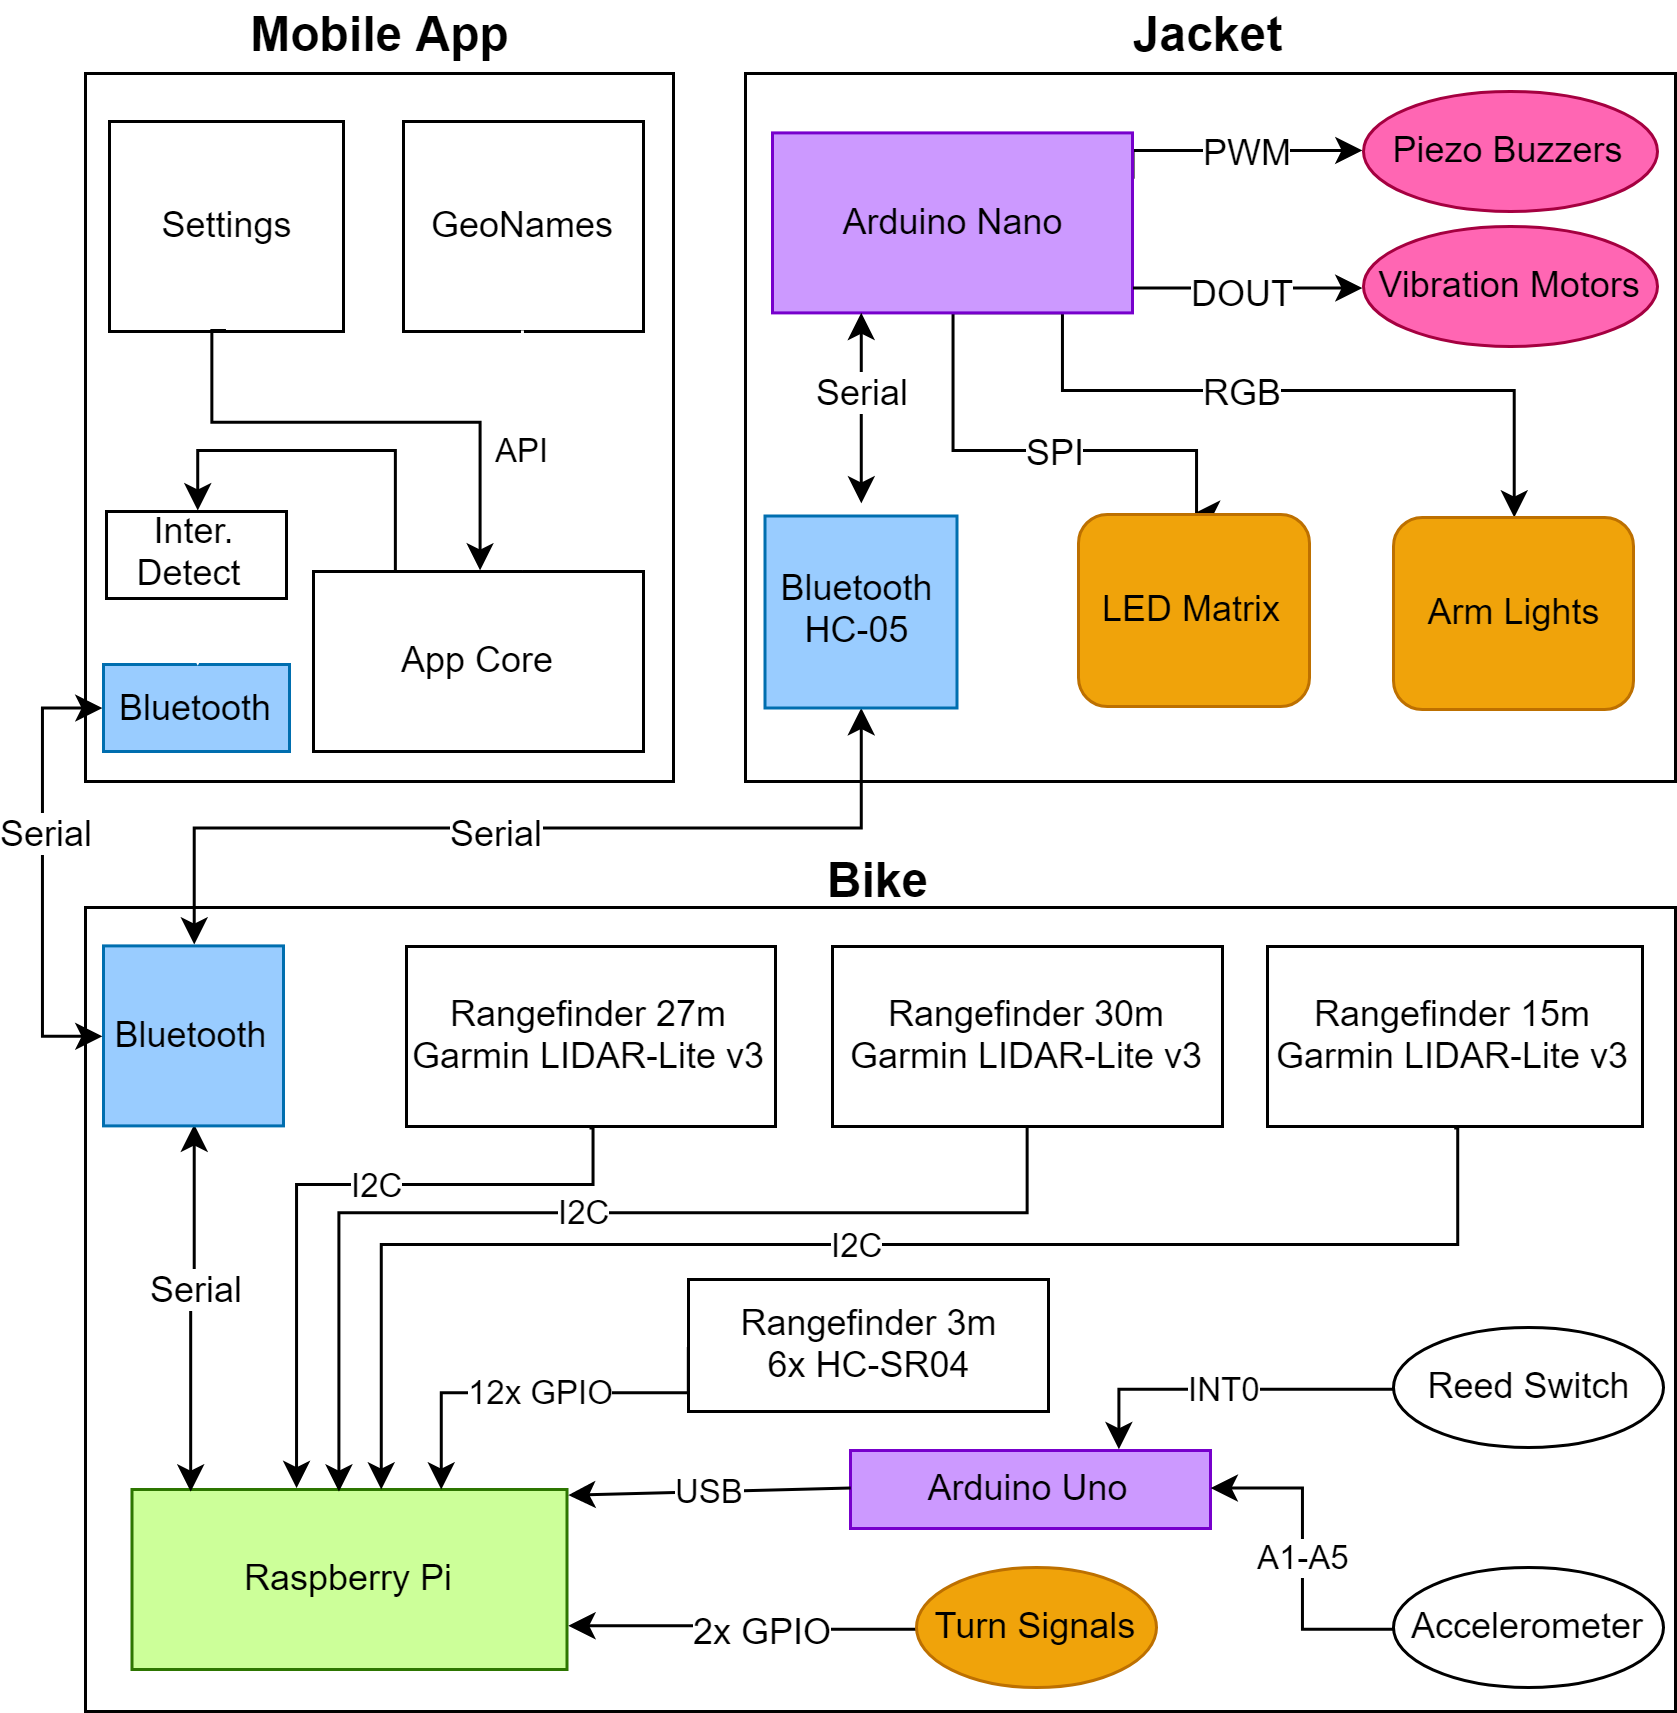
\includegraphics[width=5in]{blockdiagram}
    \caption{Block Diagram Showing the Architecture of CycleSafe}
    \label{fig:block_diagram}
\end{figure*}
\section{Architecture}
CycleSafe will consist of 3 main components,
\begin{enumerate}
    \item Mobile app that collects location and intersection data
    \item Main system mounted on bicycle that uses distance sensors and phone data to determine safety of the cyclist
    \item Jacket wearable with warning feedback and traffic lights, controlled by the main system
\end{enumerate}
The block diagram is shown in Fig.~\ref{fig:block_diagram}. In this section, we will describe what smaller devices exist on each level, and how each architectural component connects with one another.

\begin{figure}
    \centering
    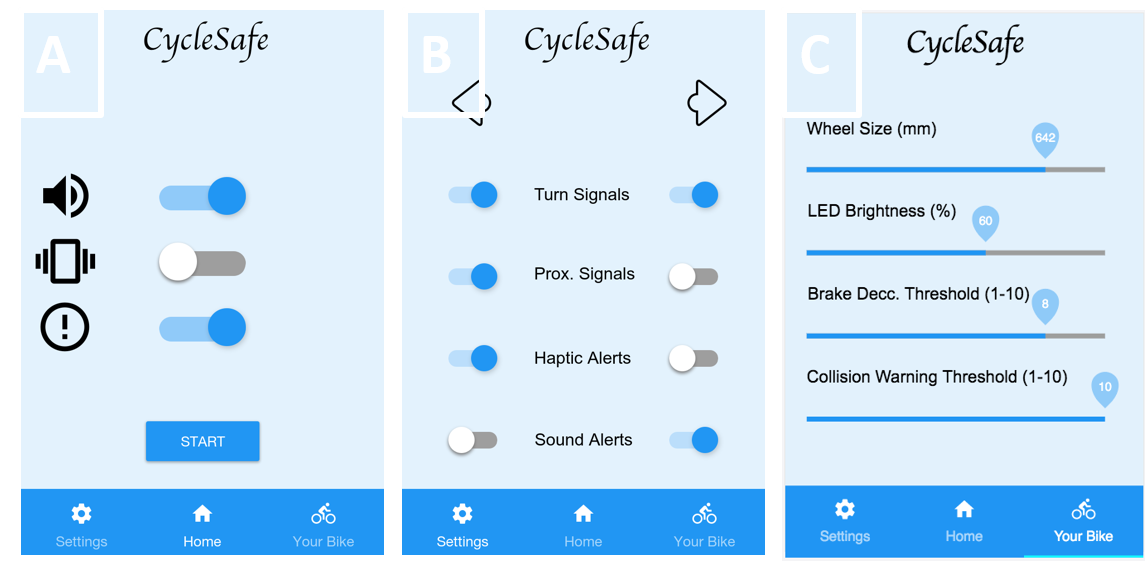
\includegraphics[width=\columnwidth]{images/app_screen.png}
    \caption{Home Screen (A), notification customization (B), threshold tuning (C)}
    \label{fig:app_screen}
\end{figure}

\subsection{Mobile App}
The mobile app is an Android application that is responsible for giving the Raspberry Pi location an intersection data, as well as providing a user interface for the user to access many features of CycleSafe, such as warning thresholds and which notification options to enable. The mobile app communicates with the Raspberry Pi via Bluetooth RFCOMM sockets. The app does not send commands directly to the jacket, but indirectly controls what shows up on the jacket by managing settings on the Raspberry Pi, which controls the main safety system on the bicycle. Screenshots of the app features can be seen on Fig.~\ref{fig:app_screen}.

\subsection{Raspberry Pi}
The bicycle will have a mounted Raspberry Pi 3 (Pi) which will be the main processing hub and run the notification and alert system. The devices connected to the Pi are as follows:
\begin{itemize}
    \item 3x \lidar{} (via I2C)
    \item 6x Ultrasonic Sensor \sonar{} (via GPIO)
    \item 2x turn signal buttons (via GPIO)
    \item Speedometer (via USB)
    \item Android Phone (via Bluetooth)
    \item Arduino Nano (via Bluetooth)
\end{itemize}
The devices connected to the Pi are meant to provide data about the bicycle status and environment, which can then be processed to determine safety conditions.

\subsection{Arduino Nano}
The Arduino Nano is the microcontroller that controls all features of the jacket, which has the following components:
\begin{itemize}
    \item 16x16 LED Matrix (output via SPI)
    \item 2x Arm LED strip warning lights (transistor control)
    \item 2x Piezo Buzzer (analog output)
    \item 4x Cell Phone Vibration Motors (transistor control with PWM power)
\end{itemize}
The Arduino has Bluetooth connection with the Raspberry Pi, where it will receive commands to give user warning feedback.

\section{Design Trade Studies}

\subsection{Vehicle Detection}
The predominant monetary cost of the CycleSafe system arises from the LIDAR rangefinders. Because of the difference in speed of motor vehicles and cyclists, sensors typical for cars cannot be used for cyclists since typical lane change sensors only check the car's blind spot, which is very close to the car, and not the region visible in the car's side mirrors. Additionally, the cost of a car makes the cost of a its safety system insignificant, but this is not the case for a bicycle since bicycles are significantly cheaper than cars. The weight requirement for a safety system is similarly far more constrained on a bicycle than on a car.

A computer-vision based vehicle and obstacle detection system was considered as a potential solution. However, we noted that the power and processing requirements of such a system and the real-time nature of the safety system would make such a computer-vision based vehicle detection system impractical. Furthermore, CycleSafe requires not only determining the location of nearby vehicles, but also to determine their speed, direction of motion, and acceleration, all of which would require processing of multiple frames at a time, increasing the processing requirements significantly. Nonetheless, a computer-vision based system would be superior in one particular situation: when detecting if vehicles are exiting side streets into the cyclist's path. This scenario is essentially impossible to address without a large number of sensors or wide-angle sensors with good resolution. However, we decided that it was worth sacrificing this scenario due to the impracticality of using such sensors or computer vision, and instead address it through signalling.

Based on these concerns, we determined that the CycleSafe system would utilize multiple single-point rangefinders that would require much less processing power to deal with. As further considerations, the CycleSafe system has to utilize longer-range sensors than in cars, and have a cost at most on the order of the cost of a bicycle. The large speed differentials between bicycles and vehicles also require higher data rates on sensors. Fortunately, there is a medium-range rangefinder commercially available. The \lidar{} has a \SI{40}{\meter} range and a measurement rate of \SI{500}{\Hz}, while weighing only \SI{38}{\gram}. It is designed for use in drones and similar real-time applications, making it well suited to CycleSafe. However, it costs \$130, which limits the quantity of these sensors the system will reasonably utilize. In designing the system, we took into account that only two or three of these sensors could be used in the entire system and that we would have to put them in strategic locations.

\label{sonar_tradeoff}
As a result, the shorter range sensors do not use the \lidar{}, but instead use the \sonar{}, a short range ultrasound rangefinder, with an effective range up to \SI{4}{\meter}. These sensors cost less than \$4, so despite their slow response time, which can be as low as \SI{20}{\Hz} and poor resolution, the CycleSafe system can utilize multiple such sensors to make up for the slow response time. In our system, we utilize 6 such sensors in order to run the proximity detection and signalling system, which only requires a range of \SI{3}{\meter}, and alternately take measurements from each sensor in order to achieve the desired update time. The redundancy proved to be important, as two of the ultrasonic sensors failed during testing but the sensing acuity of the system was not affected by them when they were disabled.

\subsection{Component Locations}

Since the CycleSafe system involves a cyclist, a bicycle and a mobile app connection, there were many decisions to make with regard to the positioning of the various components.

The rangefinder sensors could have been located on either the cyclist and the bicycle, or both. However, we decided that the potential benefits of having the sensors at a higher vantage point were outweighed by the relatively static bicycle frame as a mount, since a cyclist does not remain still when cycling.

The measurement of the cyclist's speed could have been done using either a physical measurement on the bicycle wheel or using GPS. However, due to the latency of GPS and mobile transmissions in our experience and the necessity of real-time data, it was determined that the speedometer should be physical rather than a GPS measurement.

The use of the jacket as a signalling platform rather than the bicycle was made considering the surface area and height. Since signal clarity is one of the system's primary objectives, the greater surface area of the cyclist especially when viewed from the back makes directional signals significantly clearer, as compared to the very thin profile of the bicycle viewed from behind. The added complication of needing to connect the sensor system and the signalling system wirelessly was determined to be fairly insignificant since wired communication would still be needed even if the signalling system was on the bicycle. Since the communication requirement between the sensing and the feedback system uses very little bandwidth, using Bluetooth (used in communication systems) would not increase latency significantly.

Consideration was also made as to whether the feedback system should originate from a mobile device rather than the jacket. However, we concluded that since mobile devices are actually a common cause of bicycling accidents by diverting the cyclist's attention, it would be more effective to use a platform meant solely for the safety system, which will have less potential to distract the cyclist.

\subsection{Battery Life}

Finally, in order to power all the components of CycleSafe, a battery was required. Unfortunately, batteries can be expensive in many ways, but tend to rise in price with
\begin{itemize}
    \item Smaller size
    \item Less weight
    \item Longer battery life
\end{itemize}
For CycleSafe, since we want to be as unintrusive as possible to the bicycle's overall weight so the cyclist is not slowed down, we do not want to make the system too heavy; similarly for the jacket. Fortunately, the bicycle-mounted system is very light, so most batteries are sufficiently light for the bicycle. In particular, most commuter bicycles are around \SI{30}{\lb} \cite{bicycle_weight}, and we aimed to keep our system below 10\% of the bicycle weight. Our entire bicycle-mounted system without the battery is less than \SI{1}{\lb}, so \SI{2}{\lb} of battery weight gives us plenty of options.

As for the jacket, since it is worn by the cyclist, the weight has to be significantly lighter. We estimated that if the average commuter cyclist is \SI{140}{\lb}, we wanted the jacket to be less than 5\% of the cyclists' weight, or \SI{7}{\lb}. Since the jacket and components weighs about \SI{5.5}{\lb}, we are limited to about \SI{1.5}{\lb} for the jacket battery.

In addition to the weight trade-offs, we also wanted our battery life to be long enough so that the cyclist did not have to charge the CycleSafe system too often. We deemed based on current products on the market \cite{bicycle_lights_cygolite, bicycle_lights_niterider} that 1 week was a reasonable amount of time to have the system run on a single charge.

Some options we considered for the battery to reduce cost and weight was to put a large battery on the bicycle only, and have the user plug their jacket into the bicycle. However, we thought that having a jacket attached to the bicycle would be cumbersome, and be a vulnerable point for the system to fail if it disconnected. We ended up compromising by using a medium sized power bank, the RAVPower \SI{16750}{\milli\ampere\hour} Portable Charger, for both the bicycle mount system and the jacket, one battery for each. The battery weighs \SI{0.68}{\lb}, which is under the \SI{1.5}{\lb} and \SI{2}{\lb} requirements established earlier. In addition, the capacity of the battery was tested to be around \SI{20}{\hour} for both the bicycle system and jacket, which assuming around \SI{3}{\hour} of commute time 7 days a week (which is a very high estimate), allows the cyclist to charge the system once a week.

\section{System Description}
\subsection{Android Phone}
The features of CycleSafe that are controlled through the mobile app include
\begin{itemize}
    \item \textit{Custom safety thresholds}: If the user wants to change how sensitive a safety feature is, for example collision detection, they can use sliders in the app to change how long of a notice CycleSafe will give the user a warning for.
    
    \item \textit{Custom jacket notifications}: The user can choose how they want to be notified in the event of a danger. This includes a combination of sound, light, and vibration feedback. The user can in addition choose to customize the type of vibration they feel.
\end{itemize}
In addition, the phone will provide information about when the cyclist is approaching an intersection. This is done by collecting real-time location coordinates from Google Maps API and computing the nearest intersection with help of a Geo-location API.  This is crucial, since the warning system behaves differently when the user is approaching an intersection. The phone sends intersection to the Raspberry Pi via Bluetooth.

\subsection{Raspberry Pi 3}
The Pi will be running data collection and data processing, sending commands to the Arduino Nano on the jacket. The algorithm will repeatedly run the following in its main computation loop:
\begin{enumerate}
    \item Request speed and acceleration readings from the speedometer Arduino.
    \item Request and obtain distance readings from all three LIDARs via I2C.
    \item Obtain the latest cached ultrasonic sensor readings.
    \item Check Bluetooth for incoming side-street data from Android.
    \item Perform necessary computation for blind-spot detection using the LIDAR data as well as the ultrasound data.
    \item Check the turn signals.
    \item Retrieve the speed and acceleration readings.
    \item Send warnings to Arduino Nano via Bluetooth.
\end{enumerate}

The following is done using interrupts:
\begin{enumerate}
    \item Send trigger signals out to the HC-SR04 Ultrasonic Sensors at regular intervals, with GPIO interrupts to handle the values returned.
\end{enumerate}

The primary reason the ordering is as listed above is to reduce the amount of time the Pi spends waiting. The ultrasonic sensors are the slowest sensors to respond to a measurement request. After experimental testing, the Arduino is also fairly slow to respond to a request for data over Serial, so the requests are made at the beginning and the values are retrieved only when they are needed. It was initially anticipated that the \lidar{} would have a significant response time when a request for data was made, but it was not observed to slow down the Pi computation significantly, so request and retrieval was done in immediate succession.

\begin{figure}
    \centering
    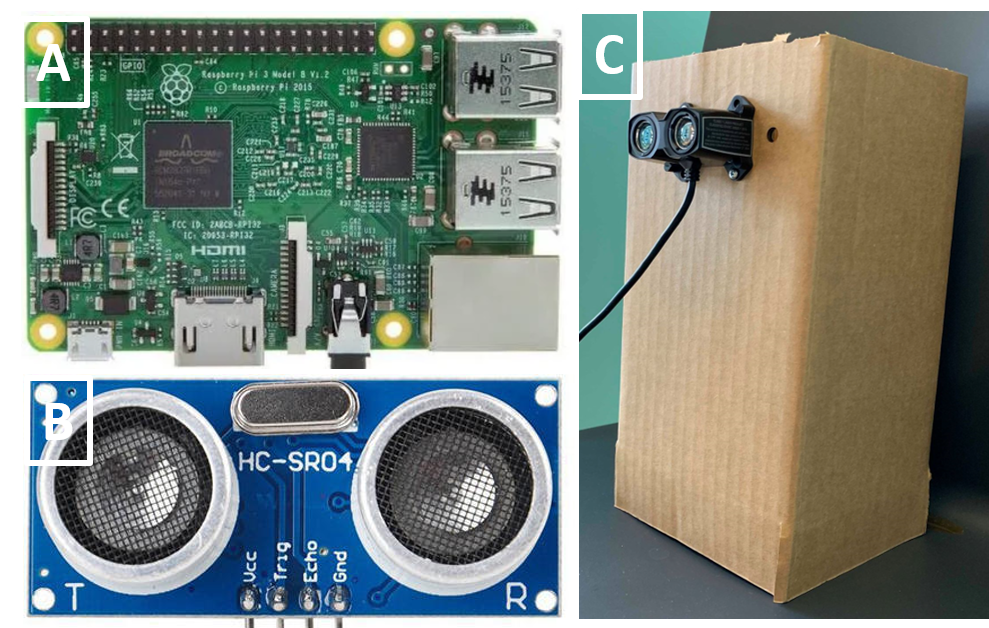
\includegraphics[width=\columnwidth]{images/rpi_range.png}
    \caption{Raspberry Pi Model 3B (A), HC-SR04 (B), Garmin LIDAR-Lite v3 (C)}
    \label{fig:rpi_range}
\end{figure}

\subsubsection{\sonar{}}

The \sonar{} is a distance sensor that uses ultrasound echolocation to figure out how far objects are away from the sensor. The device requires a trigger signal to be sent, and responds with data encoding using the length of a pulse. As such, the Pi is required to monitor the HC-SR04 echo pin when it expects a measurement to arrive. Signal-edge triggered interrupts will allow the Pi to obtain a timestamp when the pulse begins and a timestamp when the pulse ends, while still performing other useful work in the meantime. Because the ultrasonic sensors are not safety-critical for the system, they are polled at a fairly low rate, with each sensor triggered every \SI{100}{\milli\s}. To improve timing accuracy, the interrupts for returning signals are spread out over time by staggering the sensor triggers evenly over time. With six sensors, a sensor is triggered every \SI{16.7}{\milli\s}.

The processing of the raw data can then be done during the warning decision main loop, instead of the interrupt. This keeps the interrupts short and ensures they do not interfere with timing.

\subsubsection{\lidar{}}

The \lidar{} communicates with the Pi via I2C. All three rangefinders can use the same SDA/SCL lines, since they can be configured to use different I2C addresses. Experimentally, the LIDARs were found to be able to respond quickly to measurements, such that data retrieval could be done immediately after the request.

While the values obtained using the \lidar{} were fairly reliable, the sensor was also prone to noise. As such, an exponential moving average (EMA) algorithm was used to smooth out any noise from the sensor, while still allowing the system to respond fairly quickly to changes in the environment. The equation is as follows:
\begin{align}
    d_\text{curr} = \alpha d_\text{prev} + (1 - \alpha) d_\text{sample}
\end{align}
where $d_\text{prev}$ is the previous EMA adjusted reading, $d_\text{sample}$ is the latest measurement from the LIDAR, and $\alpha$ is a constant between 0 and 1. We use an $\alpha=0.75$ in CycleSafe as it allows for quick integer computation, still provides reasonable smoothing and has a quick response time to change.

\subsubsection{Warning decision algorithm}
The algorithm used by the Pi to determine what kind of warning to emit to the cyclist is described here. The severe warning is given either when the cyclist is about to collide, or something is about to collide with the cyclist. As such, severe warning will be given under the following conditions:

\begin{enumerate}
    \item The frontal sensor detects an object at a distance covered within \SI{3}{\s} at the cyclist's current speed. This warning tells the cyclist to stop or pay attention and swerve.
    \item Either of the blind-spot LIDAR sensors detect a vehicle that will overtake the cyclist within \SI{1.5}{\s} given its current velocity, and the cyclist's left turn signal is on. The warning tells the cyclist to hold their lane.
\end{enumerate}

The severe warnings are meant to be followed without the cyclist needing to consider other inputs. As such, they need to be extremely trustworthy when they are activated. In addition to false negatives, False positives must also be kept to a minimum.

The notifications are given to the cyclist under the following conditions:

\begin{enumerate}
    \item Blind spot notification: when either of the blind-spot LIDAR sensors detect a vehicle that will overtake the cyclist within \SI{2.5}{\s} given its current velocity, and the cyclist's left turn signal is on.
    \item When an intersection is approaching.
\end{enumerate}

Notifications are less critical and are mainly to keep the cyclist informed about the environment.

\subsection{Rangefinders}
\begin{figure*}
    \centering
    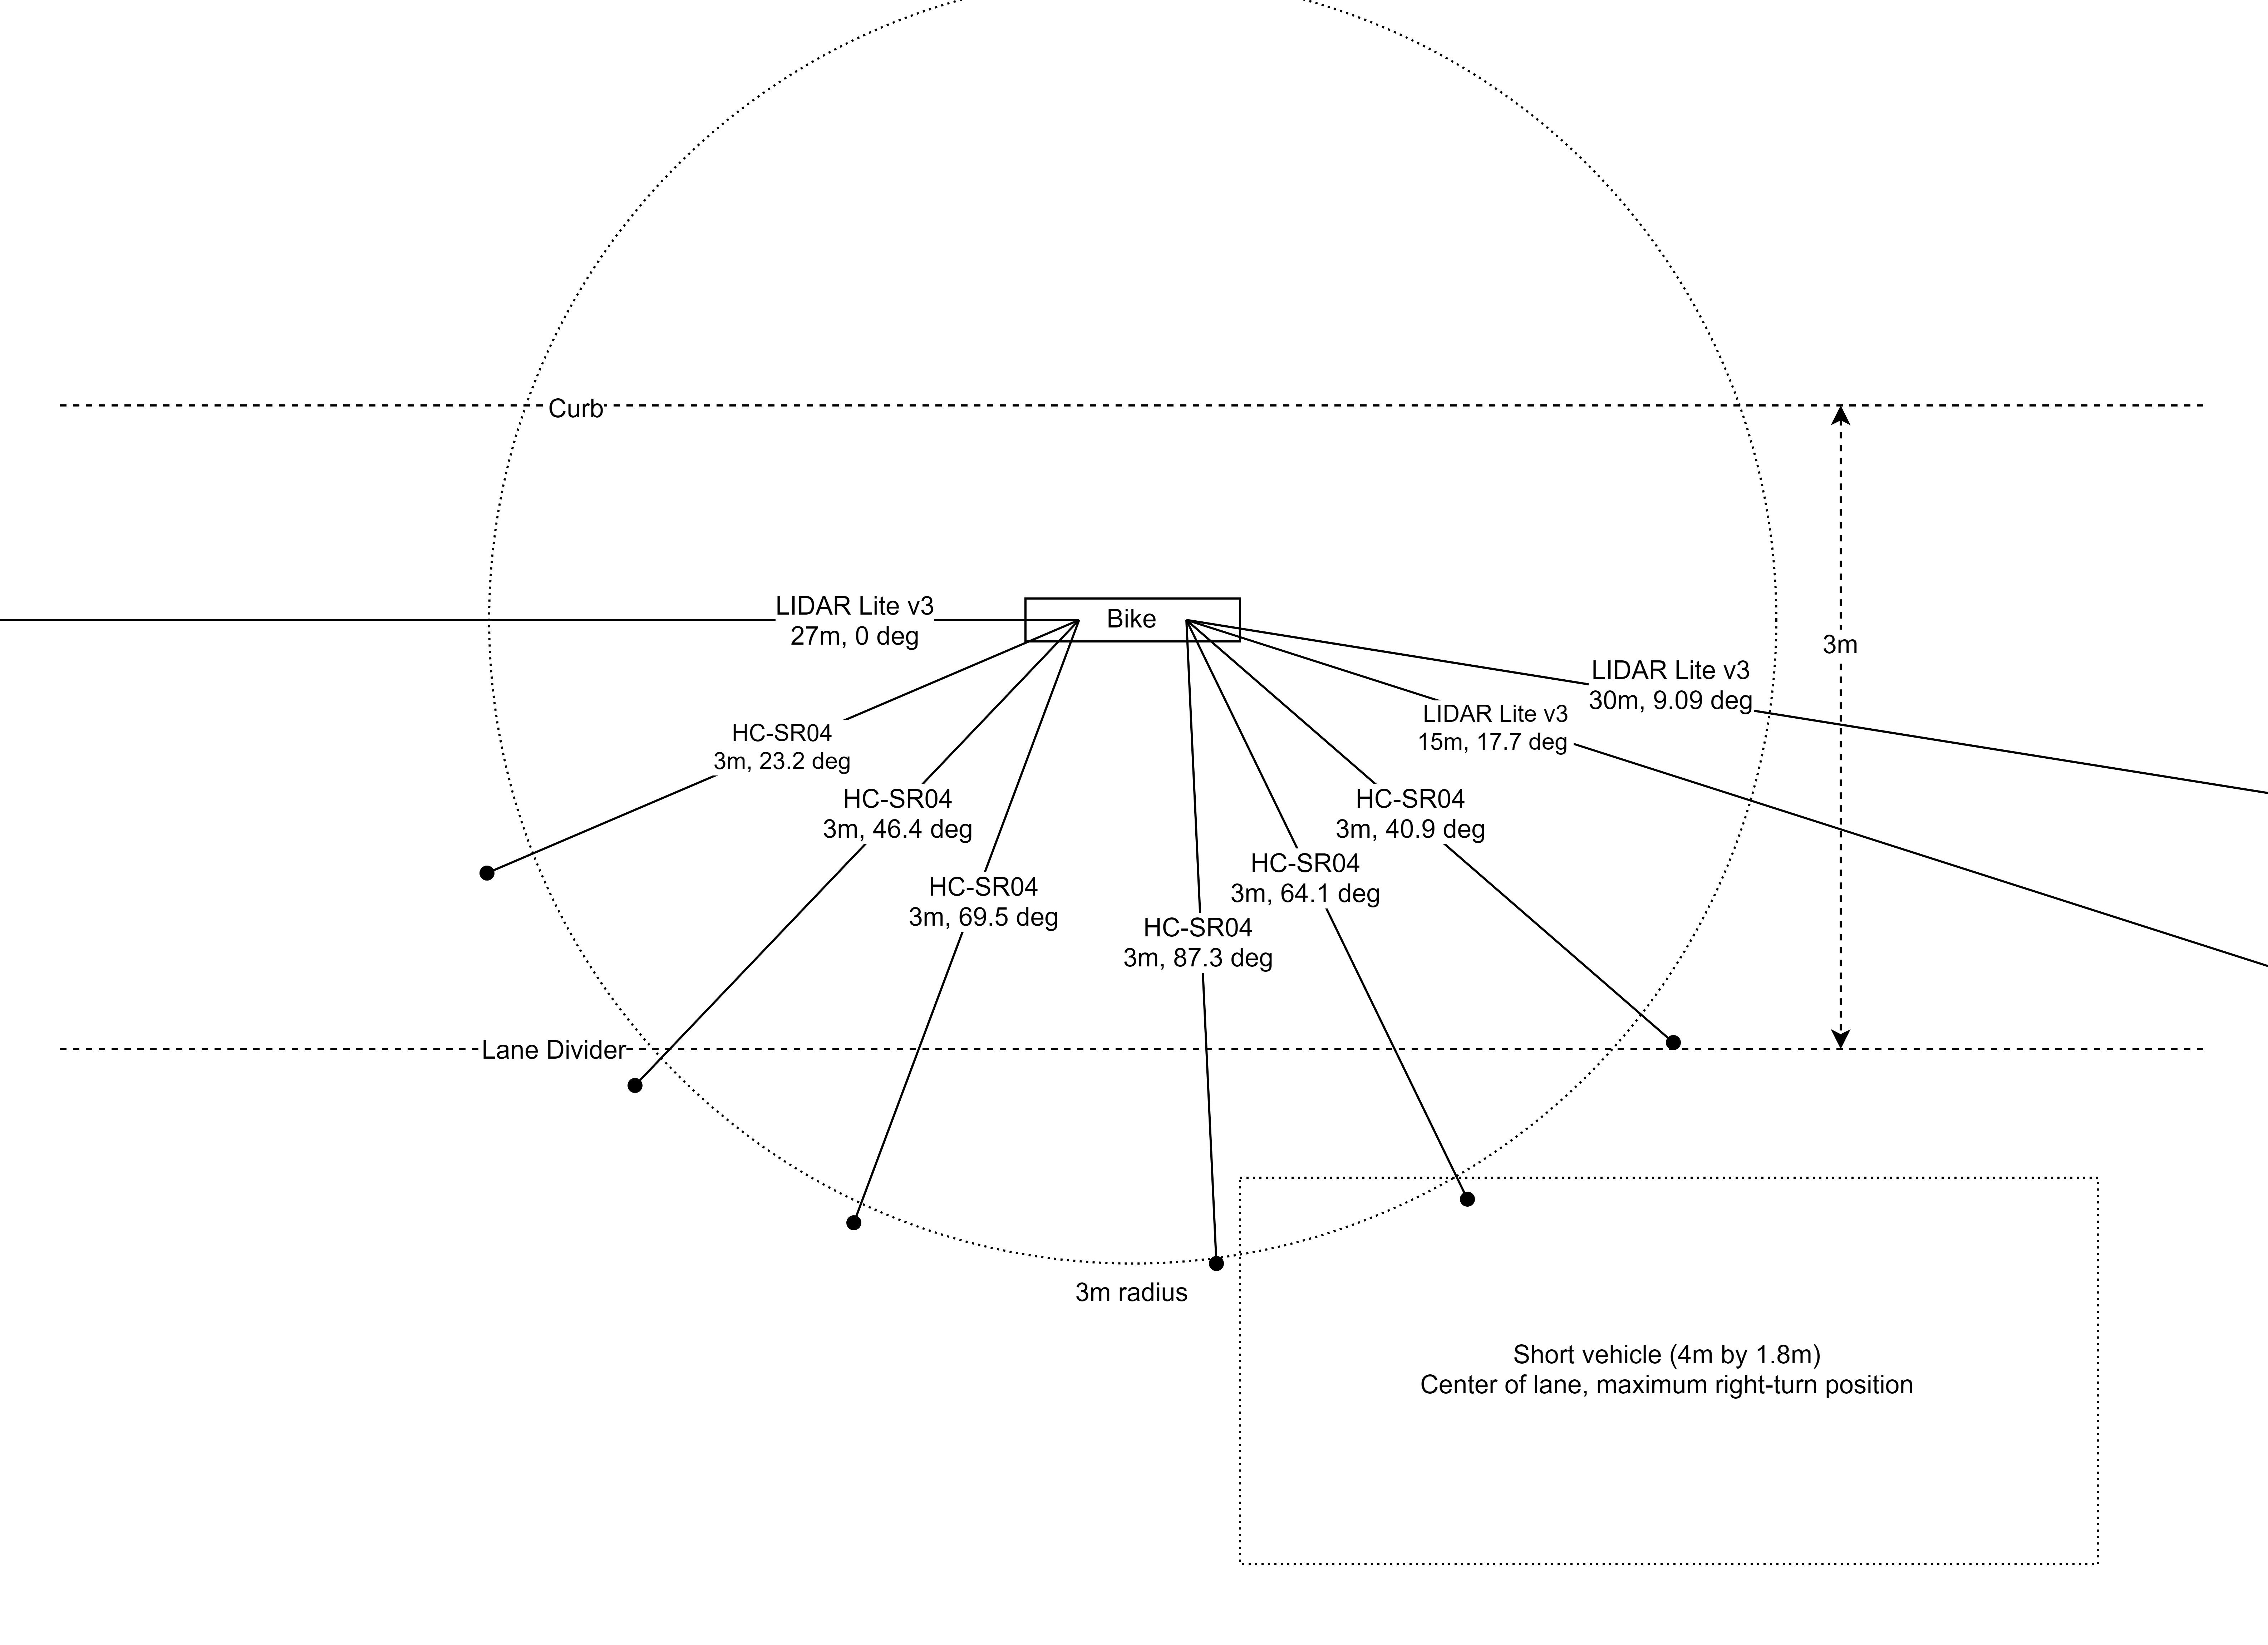
\includegraphics[width=\textwidth]{bike_config}
    \caption{Rangefinder Configuration with Bicycle Showing Ranges Covered}
    \label{fig:bike_config}
\end{figure*}
\subsubsection{Frontal sensor}
From Section \ref{specs:warning_thresholds}, we determined that the frontal sensor range requirement is at least \SI{19}{\meter}. The sensor used is a \lidar{}, which has a maximum effective range of \SI{40}{\meter}. This will be placed on a frontal mounting point on the bicycle pointing directly forward, providing unobstructed line-of-sight in front of the bicycle. It is connected directly to the Pi 3 via the 5V line and I2C bus, which will run along the length of the bicycle.

\subsubsection{Blind spot warning during lane change}
\label{sys:bswarning}
From Section \ref{specs:warning_thresholds}, we determined that the effective range of the blind spot sensor must be at least \SI{30}{\meter}. However, the blind spot sensor must face slightly diagonally in order to detect vehicles in an adjacent lane.

Given the lane width of $\slane$ = \SI{3}{\meter} and the sensor range of $s_{\text{bs\_max}}$ = \SI{30}{\meter}, we can determine the angle at which the sensor must be offset to detect a vehicle in the adjacent lane. Assuming the displacement from the cyclist to the closest point on the vehicle in the direction perpendicular to the lane direction is about one lane width, and the width of the vehicle $w_v$ is about \SI{1.8}{\meter}, we find the offset of the sensor, $\theta_{bs}$ from the axis of the direction of travel:
\begin{equation}
\theta_\text{bs} 
    = \arctan{\frac{\slane + w_\text{v}}{s_\text{bs\_max}}}
    = \arctan{\frac{4.8}{30}} 
    = \ang{9.09}
\end{equation}

Additionally we want to provide a severe warning to cyclists if it is likely that a vehicle will collide or be forced to swerve if the cyclist performs a lane change immediately. With the \SI{30}{\meter} blind spot sensor, it is well within reason to expect cars to slow down between the time they are detected \SI{30}{\meter} away and when they overtake the cyclist. However, at smaller distances a vehicle may not be in the line-of-sight of a sensor at such an acute angle. To address this, a second sensor is utilized to provide additional coverage for the blind spot, with the angle optimized to detect vehicles halfway between the longer-range sensor and the cyclist. Thus the sensor is required to have an effective range of $s_\text{bs\_near} = \SI{15}{\meter}$. Using the same method:
\begin{equation}
\theta_\text{bs\_near} 
    = \arctan{\frac{\slane + w_v}{s_\text{bs\_near}}} 
    = \arctan{\frac{4.8}{15}} 
    = \ang{17.74}
\end{equation}

\subsubsection{Right turn cut off warning}
\label{sys:cutoff}
When a vehicle is about to make a right turn into a side street in front of a cyclist, there is a large range of possible positions the vehicle may take in relation to the cyclist. However, the vehicle will always have to come into fairly close proximity to the cyclist (less than one lane width). The CycleSafe system attempts to detect this by using an array of short range sensors. These short range sensors are positioned such that any one of them will detect a compact car within one lane width to the back-left, left and front-left of the cyclist (see Fig.~\ref{fig:bike_config}). The coverage should start just outside the detection area of the \SI{15}{\meter} blind spot sensor, and extend all the way to the detection area of the frontal sensor. Generally, compact cars are at least $l_{car} = \SI{4}{\meter}$ in length. At a distance of $\slane = \SI{3}{\meter}$, the angle $d\theta_{close}$ subtended by such a car is:
\begin{equation}
\dd{\theta_\text{close}} 
    = 2\arctan{\frac{l_\text{car}}{2\slane}} 
    = 2\arctan{\frac{4}{6}} 
    = \ang{67.38}
\end{equation}

Hence, to ensure that any cars passing within the minimum distance of \SI{3}{\meter} is detected, we require a total of:
\begin{align}
    \left\lceil \frac{ \ang{180} - \ang{17.74} }{ \ang{67.38} } \right\rceil - 1 = 2
\end{align}
close proximity sensors.

However, as stated in Section \ref{sonar_tradeoff} we are using three sets of sensors, enabling staggered measurements in order to offset the slow measurement response time. This results in a total of six sensors in three sets of two each, and facing angles approximately $\ang{23}$ apart.

\subsubsection{Overall configuration}
The overall configuration of the sensors is shown in the diagram below (Fig.~\ref{fig:bike_config}). The frontal collision sensors and blind spot sensors are the \lidar{}. The six proximity sensors are the \sonar{} Ultrasonic Rangefinder.

\subsubsection{Other considerations}
It is worth noting that many laser-based range sensors typically perform more poorly in high sunlight conditions. However, this is partially compensated by the improvement in visibility and general reduction of braking distance in pleasant weather conditions.

\begin{figure}
    \centering
    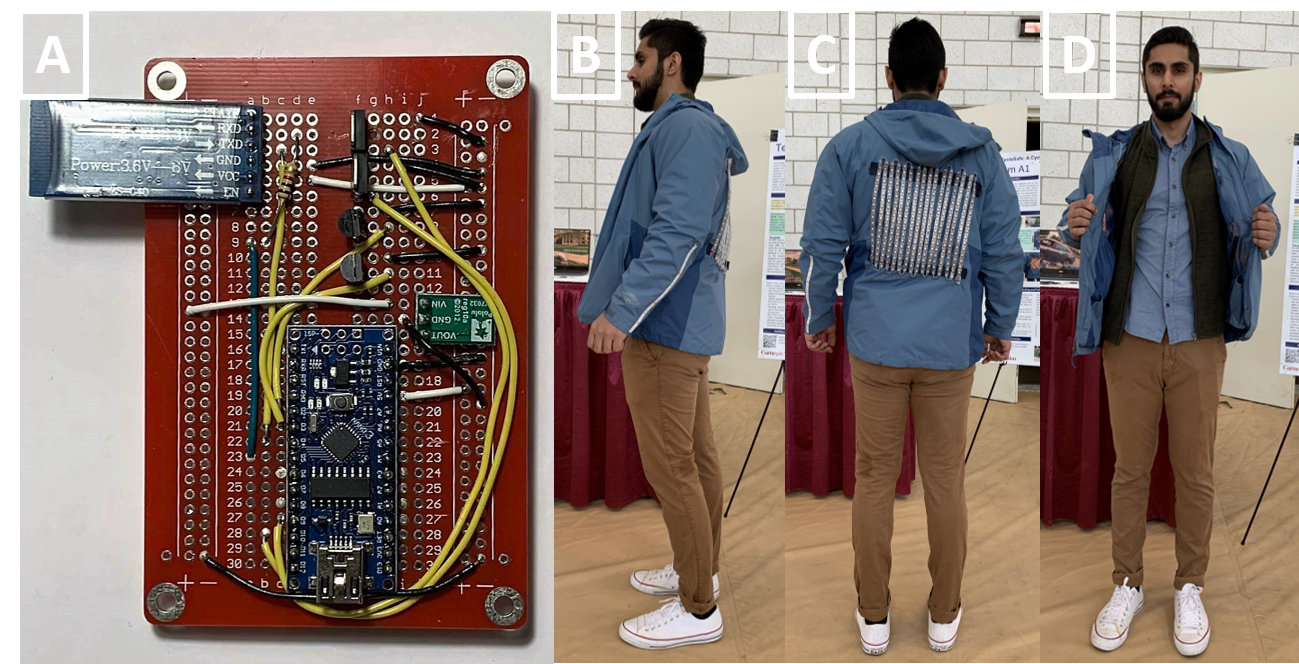
\includegraphics[width=\columnwidth]{images/jacket_chip.png}
    \caption{On Jacket Chip (A), views of the jacket (B, C, D)}
    \label{fig:jacket_chip}
\end{figure}

\subsection{Arduino Nano}
The Arduino Nano is the microcontroller that is responsible for controlling all the peripherals on the jacket. More details about each individual component can be found in the following sections. Since the jacket does not send any data to the Raspberry Pi, it is a passive component in the architecture, and thus the Nano only receives commands via Bluetooth from the Raspberry Pi. 

We built a custom chip for the Arduino Nano (see Fig.~\ref{fig:jacket_chip}.A) to condense the circuitry in the jacket to be very small and fit well. Some notable components on the chip are
\begin{itemize}
    \item \textit{Arduino Nano:} microcontroller to control all peripherals
    \item \textit{Bluetooth chip:} used for communication between the Nano and the Pi
    \item \textit{MOSFETs:} used to control high power devices 
    \item \textit{5V to 12V step-up converter:} to power the proximity lights, which are 12V LEDs instead of the 5V LEDs that make up the LED matrix
\end{itemize}

\subsection{LED Matrix}
The LED Matrix serves as the main light signalling component of the jacket wearable. Similar to how cars have turn signals and brake lights, the LED Matrix in the back can serve any of these light functions. We are using WS2812B LED strips, which have individually addressable LEDs, so thus the matrix is configurable to its $16 \times 16$ granularity and 8-bit RGB, and therefore can emulate almost any signal. 

For our project, the LED Matrix has the following lighting modes,
\begin{itemize}
    \item \textit{Ambient lights:} Matrix is a dim red, at approximately \SI{50}{\milli\candela}. This mode is important during nighttime, to give other vehicles constant awareness of the rider. 
    \item \textit{Brake lights:} Matrix is a brighter red than the ambient light, at \SI{300}{\milli\candela}. This mode is triggered if the speed of the rider is slowing down. 
    \item \textit{Turn Signals:} Flashing arrows that indicate the direction in which the cyclist is trying to turn. Brightness of \SI{300}{\milli\candela}.
\end{itemize}

In order to display images on the LED Matrix, 2D data has to first encoded into 1D linear data, and then to the LED strip serially. The Arduino has code that serializes LED matrix image data. To make the image drawing on the LED matrix quick, there are preset images, which are triggered by the Raspberry Pi through the communication protocol, instead of having the Raspberry Pi draw each image one LED at a time.

\subsection{Proximity Lights}
There are proximity lights on the sides of both arms, facing outwards from the riders. These lights notify drivers when they are near the cyclist, so that they are more aware of the cyclist. The proximity lights are implemented using waterproof SMD5050 RGB strips, which are not addressable, and controlled directly with DC voltage. See Fig.~\ref{fig:buzz_motor_prox}.C.

\subsection{Piezo Buzzers and Vibration Motors}
One feature of CycleSafe is to give the rider as much awareness about the road as possible, while also allowing the rider to focus on the road by keeping the system minimally intrusive. The piezo buzzers and Vibration Motors are forms of non-visual feedback to the rider, namely auditory and sensory respectively, that use beeping sounds and vibrations to give the rider warning about dangerous situations.

This is akin to how many blind spot features in cars nowadays beep when a driver is about to turn into a lane that is not empty. This type of feedback is very important, because people can forget to check that a lane is empty before changing. In addition, for a cyclist who has no rear or side mirrors, they have to expend a larger motion just to check if a lane is clear. Therefore, these two forms of feedback minimize the need for the rider to check for visual warnings, and also serves as a fallback warning system in case the rider just forgets to check in the first place.

\begin{figure}
    \centering
    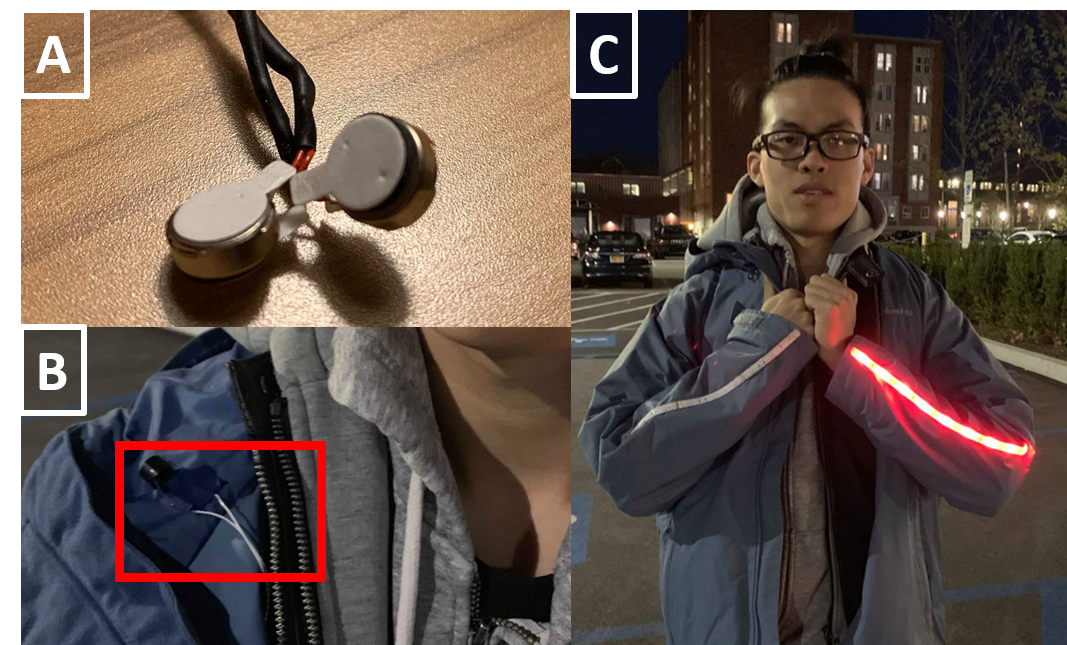
\includegraphics[width=\columnwidth]{images/buzzer_motor_prox.png}
    \caption{Views of vibration motors (A), piezo buzzer (B), proximity lights (C)}
    \label{fig:buzz_motor_prox}
\end{figure}

The two piezo buzzers have different pitches, where the higher pitched one indicates frontal collision danger. The piezo buzzers are positioned on the collar of the jacket, which is close enough for the rider to hear distinctly even in the loud environment of the road. There are two sets of vibration motor packs, each pack contains two motors. These vibration motors are placed on the shoulder of the jacket, to emulate a ``tap on the shoulder''-like sensation.

\subsection{Speedometer}
The function of the speedometer is to determine the speed of the bicycle. It consists of a single reed switch, placed on the bicycle's front fork, activated by a magnet, and connected to the interrupt pin on the Arduino Uno. The circuit is shown in Fig.~\ref{fig_speedometer}.

\begin{figure}[!t]
\centering
    \def\cktWidth{4}
    \def\rHeight{4}
    \def\rWidth{2.5}
    \def\rA{3.5}
    \def\rB{2}
    \def\rC{0.5}
    \begin{circuitikz}
        % \tikzmath{\r_height = 4; \r_width=3;}
        \draw (0,0) rectangle (\rWidth,\rHeight) node[yshift=-12pt, pos=0.5, label={[align=center]Arduino Uno}] {};
        
        \node (5V) at  (\rWidth + 1, \rA) {\SI{5}{\volt}};
        \node (GND) at (\rWidth + 1, \rB) {GND};
        \node (D2) at  (\rWidth + 1, \rC) {D2/INT0};

        \draw (\rWidth, \rA) 
            to[short] (5V.west)
            to[open]  (5V.east)
            to[ospst]  (\rWidth + \cktWidth, \rA)
            to[short] (\rWidth + \cktWidth, \rC)
        ;
        
        \draw (\rWidth, \rB) 
            to[short] (GND.west)
            to[open]  (GND.east)
            to[R=$\SI{10}{\kilo\ohm}$]  (\rWidth + \cktWidth, \rB)
        ;
        
        \draw (\rWidth, \rC) 
            to[short] (D2.west)
            to[open]  (D2.east)
            to[short]  (\rWidth + \cktWidth, \rC)
        ;
    \end{circuitikz}
\caption{Speedometer circuit configuration.}
\label{fig_speedometer}
\label{fig_speedometer_1}
\end{figure}

The speedometer will require the user to configure the wheel diameter or the wheel circumference using the app interface. The bicycle velocity, $v_b$ will then be computed by the Arduino Uno, as follows:
\begin{equation}
    v_b = \frac{4\pi d}{t - t_{4}}
\end{equation}

where $t$ is the current timestamp, $t_{4}$ is the timestamp four interrupts prior, and $d$ is the diameter of the wheel. Wheel diameters typically range from \SI{507}{\milli\m} to \SI{622}{\milli\m}, with \SI{622}{\milli\m} being the most common \cite{bike_wheel_size}.

Waiting for four interrupts computes the average speed over the last four wheel rotations instead of merely the last rotation. This reduces speed fluctuations, which would adversely affect the accuracy of the warning algorithm. It also reduces the error in case an interrupt is missed or an additional interrupt somehow occurs. in this case, the average of four limits the error to 25\% of the actual value. An average of four was used because four rotations of a \SI{622}{\milli\meter} wheel on a bicycle covers a distance of \SI{7.816}{\m}, which is approximately one second at typical bicycle speeds of \SI{5}{\meter/\s} to \SI{9}{\meter/\s}. However, the trade-off is that the it may take up to a second for the speedometer to respond to changes in velocity. Large changes in speed are only likely when the bicycle is coming to a sudden stop, and therefore a slower response to a sudden decrease in speed will favor false positives over false negatives, which is preferable.

\begin{figure}
    \centering
    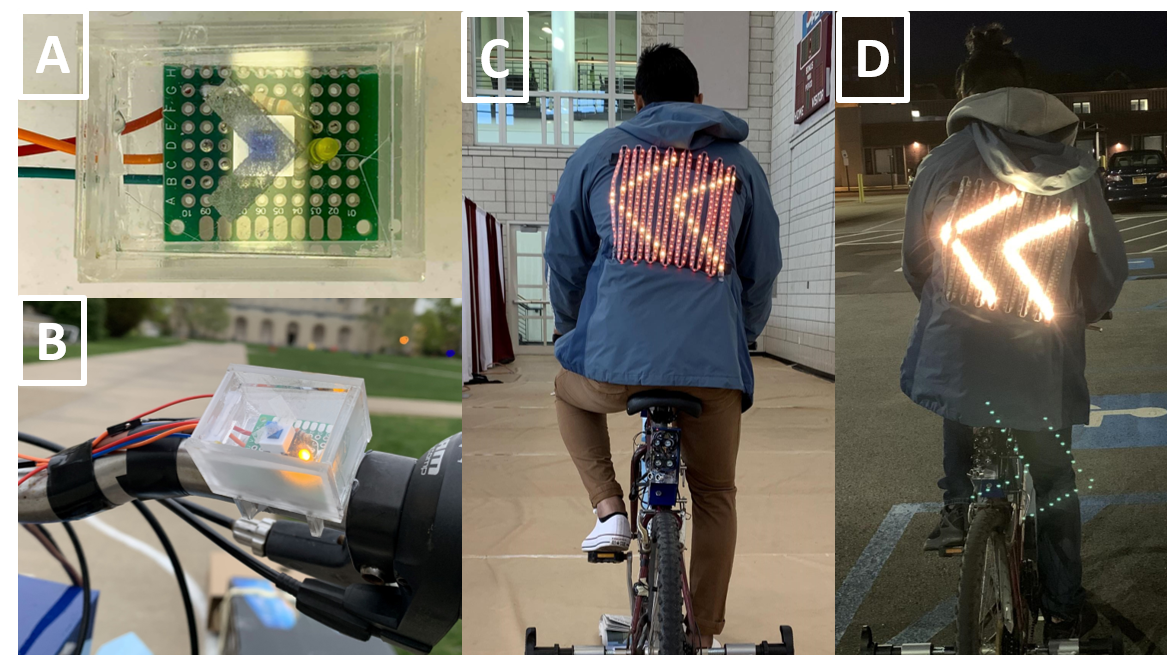
\includegraphics[width=\columnwidth]{images/turn_signals.png}
    \caption{Turn signal profile (A), turn signal on (B), matrix in daytime (C), matrix in nighttime (D)}
    \label{fig:turn_sig}
\end{figure}

\subsection{Turn Signals}
To give users the ability to display turn signals on their LED matrix, there are turn signal buttons on the bicycle. These are simple push-latch buttons, that light up when they are pressed so the user knows when the turn signals are on.
The pictures for the turn signals and their LED matrix display are shown in Figure~\ref{fig:turn_sig}.

In addition to just enabling turn signals the buttons also have other functions. The full list is
\begin{itemize}
    \item \textit{Left Turn Signal Only}: Left turn signal is on
    \item \textit{Right Turn Signal Only}: Right turn signal is on
    \item \textit{Left and Right Turn Signal Held for $<\SI{5}{\s}$}: CycleSafe toggles ambient lighting mode, where the LED matrix is kept either off or on dim by default.
    \item \textit{Left and Right Turn Signal Held for $\geq\SI{5}{\s}$}: CycleSafe performs a system restart.
\end{itemize}

\begin{figure}
    \centering
    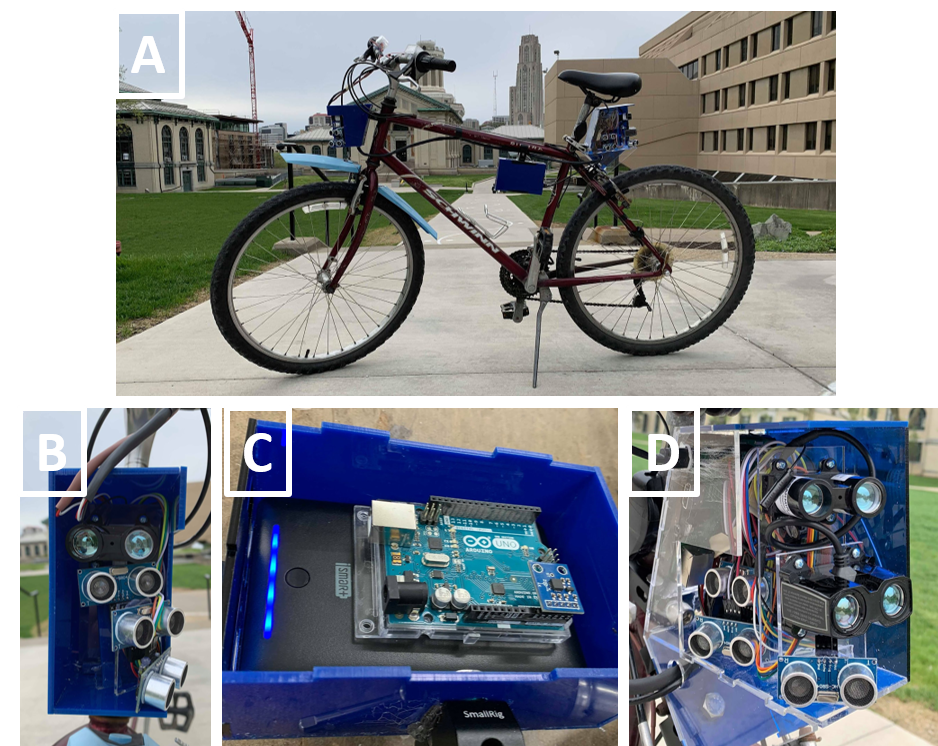
\includegraphics[width=\columnwidth]{images/bike_mount.png}
    \caption{Mount for the Bicycle (A), front sensors (B), battery and speedometer Arduino (C), back sensors (D)}
    \label{fig:bike_mount}
\end{figure}

\subsection{Bicycle Mount}
To put all the rangefinders, ultrasonics, speedometers, and other sensors onto the bike at the precise angles specified, we had to construct mounts onto the bicycle. These mounts were created in Solidworks and laser-cut to precisely meet the design specifications.

The setup for the bicycle mounts are shown on Fig.~\ref{fig:bike_mount}. There are three main boxes that are mounted onto the bike
\begin{itemize}
    \item \textit{Front Sensors:} The front box has one LIDAR sensor for frontal collision detection, and three HC-SR04 ultrasonic sensors for adjacent lane detection.
    \item \textit{Middle Box:} The middle box holds the Arduino that is dedicated to collecting accelerometer and speed data from the reed switch. The box also contains the battery that powers the entire bike system. 
    \item \textit{Back Sensors:} The back box has two LIDAR sensors for blind spot danger detection, and three HC-SR04 ultrasonic sensors for adjacent lane detection. The back also houses the Raspberry Pi. The back box is the hub for all control, and is connected to the front box via a bus that runs along the bike.
\end{itemize}

\section{Project Management}
All of the source code for our project can be found at our \href{https://github.com/mikinty/CycleSafe}{\underline{Github repository}}. In addition, Solidworks models for the casing can be found in the repository as well. Other image and video data was stored on Google Drive, and not shared publicly.

\subsection{Schedule}
We used TeamGantt to organize our tasks and keep track of our progress. We have attached our Gantt Chart schedule at the end of the paper. 

We finished every task that we originally set in the beginning of the project, so our planning was a big success. 

A link to our TeamGantt chart can be found \href{https://prod.teamgantt.com/gantt/schedule/?ids=1489092&public_keys=7aQHatcI23su&zoom=d100&font_size=12&estimated_hours=0&assigned_resources=0&percent_complete=0&documents=0&comments=0&col_width=355&hide_header_tabs=0&menu_view=1&resource_filter=1&name_in_bar=0&name_next_to_bar=0&resource_names=1#user=&company=&custom=&date_filter=&hide_completed=false&color_filter=}{\underline{here}}.

\subsection{Team Member Responsibilities}
% not sure how we want to structure this, could just do 3 sections
\textbf{Benjamin}
\begin{itemize}
    \item Raspberry Pi control software
    \item Interfacing between the Pi and bike components: LIDARs, ultrasonics, speedometer, accelerometer
    \item Logic for safety conditions
\end{itemize}

\textbf{Siddhanth}
\begin{itemize}
    \item Develop the mobile app, including Bluetooth communication, map API development, UI
    \item Write intersection detection algorithms
    \item Collect bike location and intersections to send as inputs to the safety logic in the Raspberry Pi
\end{itemize}

\textbf{Michael}
\begin{itemize}
    \item Modify a jacket to have an LED matrix, proximity lights, piezo buzzers, and vibration motors, with waterproofing
    \item Create custom jacket chip to integrate jacket peripherals with the Arduino Nano controller
    \item Design and create jacket lights to satisfy official vehicle
requirements
    \item Design and construct the bicycle mounts that house all bike components and sensors
\end{itemize}

\textbf{All}
\begin{itemize}
    \item Design a Bluetooth communication protocol between devices
    \item Conduct safety tests to measure system robustness
\end{itemize}

\subsection{Budget}
\begin{table}[H]
    \centering
    \begin{tabularx}{0.4\textwidth}{ll}
        \toprule
         \textbf{Item}  & \textbf{Price}  \\
         \midrule
         % Bike
         Garmin LIDAR-Lite v3-HP        & \$149.99\\
         Garmin LIDAR-Lite v3 (2)       & \$129.99 each\\
         HC-SR04 Ultrasonic Sensor (6)  & \$6.99 each\\
         EK1621x2 Reed Switch           & \$0.50\\
         ADXL335 Accelerometer          & \$14.95\\
         $1' \times 1'$ Acrylic Piece (3) & \$2.20 each\\ 
         SMALLRIG Super Clamp (4)$^\ast$       & \$7.99 each\\
         
         % Jacket
         WS2812B LED Strip              & \$28.95\\
         SMD5050 LED Strip (1 ft)       & \$0.74 per ft\\
         Piezo Buzzer PS1240 (2)        & \$1.50 each\\
         Cellphone Vibration Motor (4)  & \$1.95 each\\
         HC-05 Bluetooth Module         & \$4.99\\
         
         % control
         Raspberry Pi Model 3 $^\ast$          & \$29.99\\
         Arduino Nano $^\ast$                  & \$4.95\\
         
         % Power
         16750mAh Portable Charger (2)     & \$34.99 each\\
         \midrule
         \textbf{Total (without $^\ast$)} & \textbf{\$589.42}\\
         \textbf{Grand Total} & \textbf{\$656.32}\\
         \toprule
    \end{tabularx}
    \caption{Prices for materials. Materials marked with $^\ast$ were paid out-of-pocket.}
    \label{tab:prices}
\end{table}

\subsection{Risk Management}
Having parts come in late was expected, but we fortunately had many of the major parts already in hand, we could develop without some of the parts coming in. For example, we already had a Raspberry Pi, Arduino Nano, and a mobile phone at the start of the project, so we could develop on those devices while waiting for our other parts to come in. 

One of the major concerns we had for our entire system was power, since we eventually wanted to have a portable power source and we had some potentially power-consuming devices, including LED strips and LIDAR sensors. To reduce risk, we did two things
\begin{enumerate}
    \item Reduce the power consumption of these devices. For the LED strips, we made sure to only activate a subset of the 256 available lights. For the LIDAR, we only requested for distance data when we needed it.
    \item Put more batteries on the bike, and plug in the jacket into the bike as a backup option for power.
\end{enumerate}

%%% TESTING IMAGES %%%
\begin{figure}
    \centering
    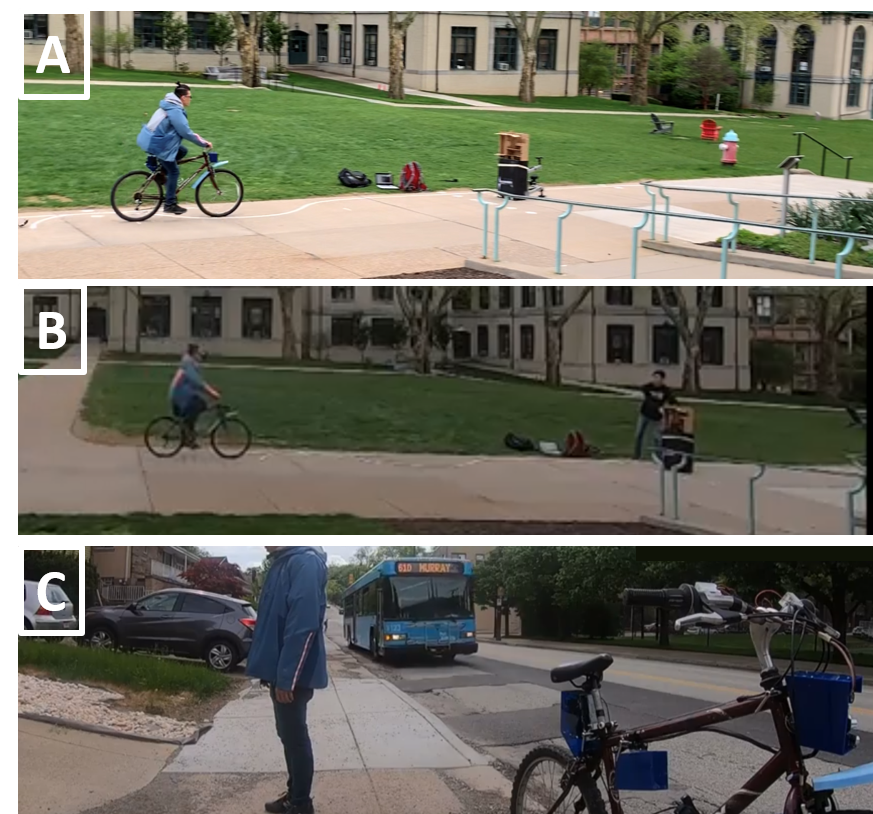
\includegraphics[width=\columnwidth]{images/blind_collision_tests.png}
    \caption{Frontal collision test (A), sudden obstacle collision (B), blind spot warning (C)}
    \label{fig:collision_blind}
\end{figure}

\begin{figure}
    \centering
    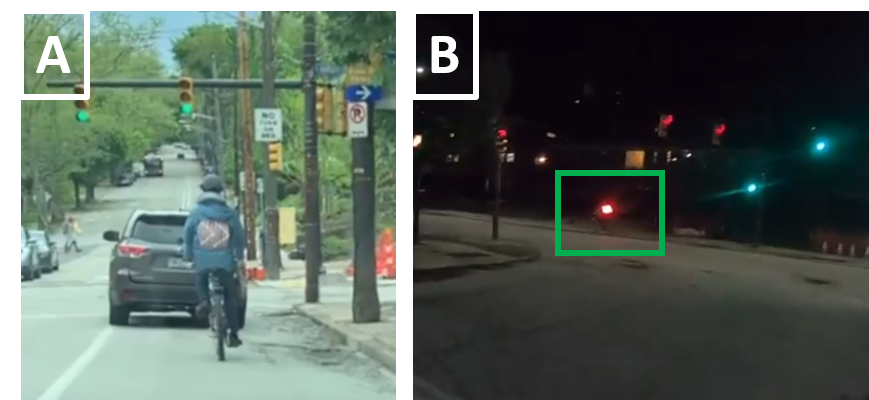
\includegraphics[width=\columnwidth]{images/visibility.png}
    \caption{LED matrix signal visibility at daytime (A), nighttime (B)}
    \label{fig:visibility}
\end{figure}

\begin{figure}
    \centering
    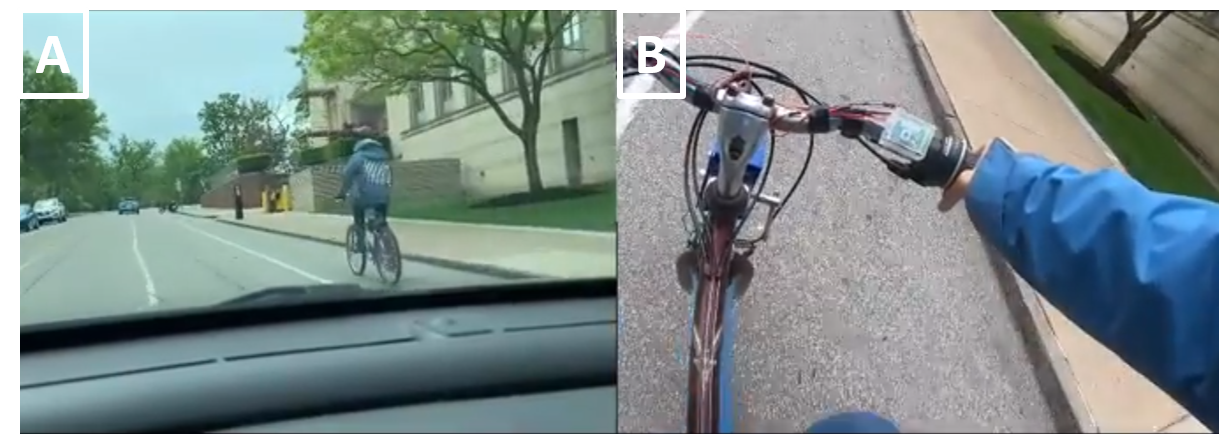
\includegraphics[width=\columnwidth]{images/side_by.png}
    \caption{Overtaking the cyclist from the car view (A), cyclist view (B)}
    \label{fig:overtake}
\end{figure}

\section{Testing Results and Discussion}
The results obtained from testing the system in the field are as follows:

\begin{table}[H]
    \centering
    \begin{tabularx}{0.8\columnwidth}{|X|c|}
        \hline
        \textbf{Test} & \textbf{Successful/Total} \\ \hline
        Frontal collision & 4/13 \\ \hline
        Sudden obstacle & 6/7 \\ \hline
        Obstacle (false positive) & 10/10 \\ \hline
        Blind spot & 4/10 \\ \hline
        Blind spot (false positive) & 16/39 \\ \hline
        Proximity & 6/6 \\ \hline
    \end{tabularx}
    \vspace{6pt}
    \caption{Testing results}
    \label{table-results}
\end{table}

\subsection{Frontal collision tests}
The frontal collision testing data (Fig.~\ref{fig:fc1}) indicates that the system provides about \SI{2}{\s} of alert lead-time below \SI{5}{\meter/\s}, and about \SI{1.5}{\s} of alert lead-time at higher speeds, with a minimum of \SI{1}{\s}. This is not as much as we initially wanted at the higher speeds, however it still provides enough time for the cyclist to swerve, since during testing the cyclist only swerved after the alert was active but never collided with the dummy obstacle.

\begin{figure}
    \centering
    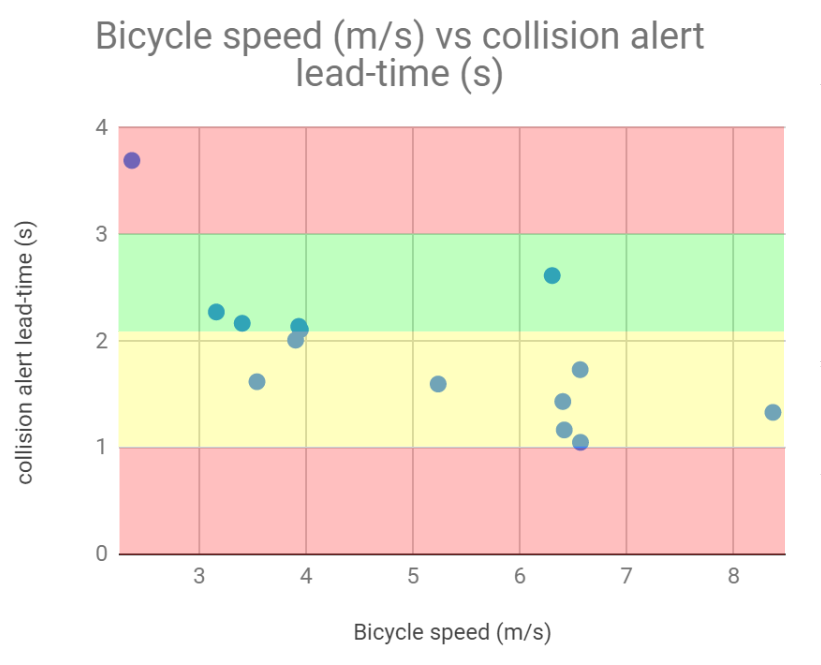
\includegraphics[width=\columnwidth]{FC1_lt.png}
    \caption{Frontal collision testing data. Green region is the braking region. Yellow region is the swerving region.}
    \label{fig:fc1}
\end{figure}

Various reasons are responsible for the lower-than-expected lead-time. The frontal LIDAR sensor was not always aligned exactly to face the obstacle due to bumps in the road, slight road curvature, and similar reasons. Any deviation away from the obstacle would cause the LIDAR to report distances much further than the obstacle (which pose no danger to the cyclist), causing the system not to alert the cyclist. Using lower alpha-values in the exponential moving average error-correction and smoothing algorithm for calculating distance to obstacle would result in better response in this scenario, but also more false positives due to noise, which would reduce the cyclists' trust in the system.

With regard to sudden obstacle detection (Fig.~\ref{fig:fc2}), the average response-time-to-alert fell well below the \SI{0.9}{\s} requirement, at \SI{0.66}{\s}. The worst-case test had a response-time-to-alert of \SI{0.96}{\s}, only 7\% higher than the desired threshold. Given that the tests were done almost exactly as would happen in a realistic scenario with many external factors that would affect response time, this test is very successful.

\begin{figure}
    \centering
    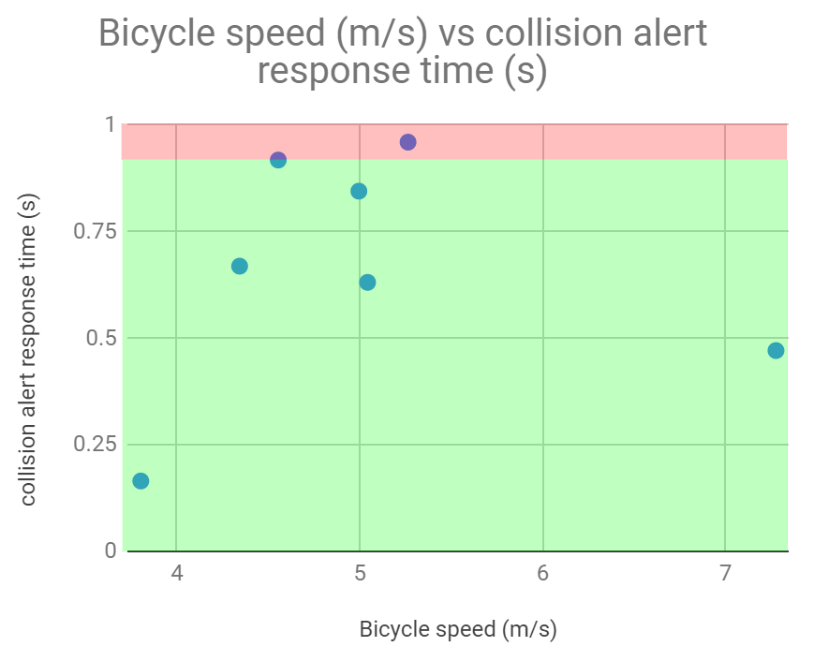
\includegraphics[width=\columnwidth]{FC2_rt.png}
    \caption{Sudden obstacle testing data. Green region is an improvement on human perception time.}
    \label{fig:fc2}
\end{figure}

Finally, the false positive test, with obstacles moving away from the system, performed outstandingly. Except for the alert when the obstacle is initially brought into the cyclists' path, there was no other time that alerts were activated during the test.

\subsection{Blind spot tests}
In general, the blind spot tests performed reasonably well in spite of a number of potential sources for error. The tests were carried out along Forbes Avenue which runs through Carnegie Mellon University, using real traffic for testing. This allowed a large amount of extremely realistic data to be collected for a variety of vehicles, distances and speeds.

For the blind-spot alert test conditions, the alert results are very promising (Fig.~\ref{fig:bs1_buzz}). The tests were filtered to find all instances of vehicles passing within \SI{2.5}{\meter} of the bicycle, obtaining 10 scenarios. Of 10 scenarios, all alerts were generated within \SI{0.5}{\s} for vehicle speeds between \SI{7}{\meter/\s} \SI{11}{\meter/\s} (8 of 10 tests), with the minimum lead-time being \SI{0.793}{\s}. The remaining two tests have vehicle speed between \SI{14}{\meter/\s} and \SI{15}{\meter/\s}, have an alert time of \SI{0.387}{\s} and \SI{0.434}{\s}. While this does not fall within the requirements we originally wanted, this is very close to the maximum speed at which we want the system to give a guarantee. 9 of 10 tests do not alert earlier than the stipulated \SI{1.5}{\s}, meeting the requirement. In 1 of the tests the alert activated \SI{2.2}{\s} before the vehicle passes the bicycle. This was a fairly slow vehicle moving at \SI{7.27}{\meter/\s}.

\begin{figure}
    \centering
    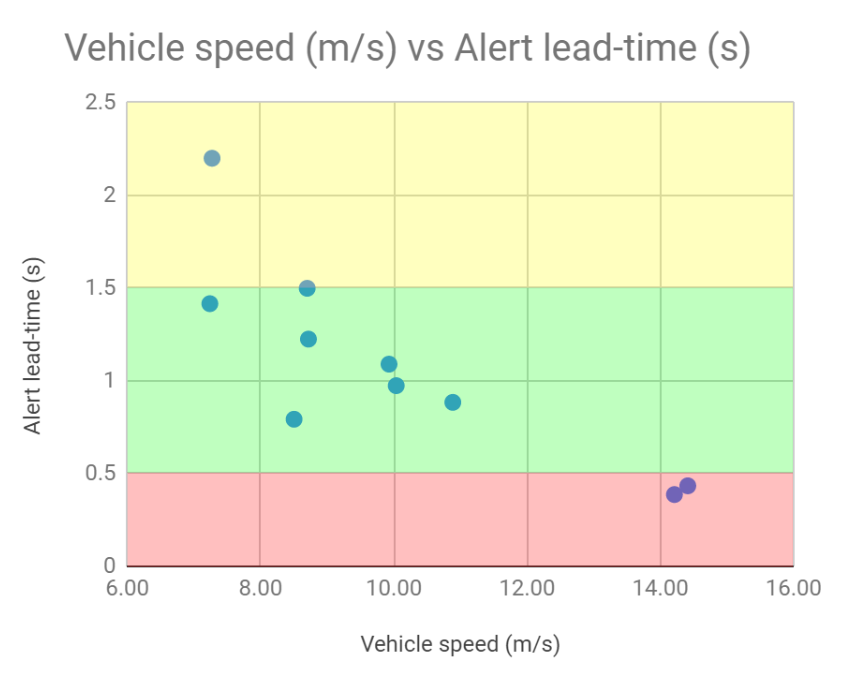
\includegraphics[width=\columnwidth]{images/BS1_buzz.png}
    \caption{Blind spot alert testing data. Green region meets the specification. Yellow region is an early alert.}
    \label{fig:bs1_buzz}
\end{figure}

The notifications, however, did not come as early as we initially required (Fig.~\ref{fig:bs1_vib}). 4 of 10 tests have notification lead-time earlier than \SI{1.5}{\s}, all of which have vehicle speed below \SI{9}{\meter/\s}. 4 other tests have notification lead-time between \SI{0.8}{\s} and \SI{1.5}{\s}, with vehicle speeds between \SI{8}{\meter/\s} and \SI{12}{\meter/\s}. Finally, the remaining 2 tests are the the aforementioned high-speed vehicles, which have notification lead-time of \SI{0.387}{\s} and \SI{0.451}{\s}, approximately the same as their alert lead-time.

\begin{figure}
    \centering
    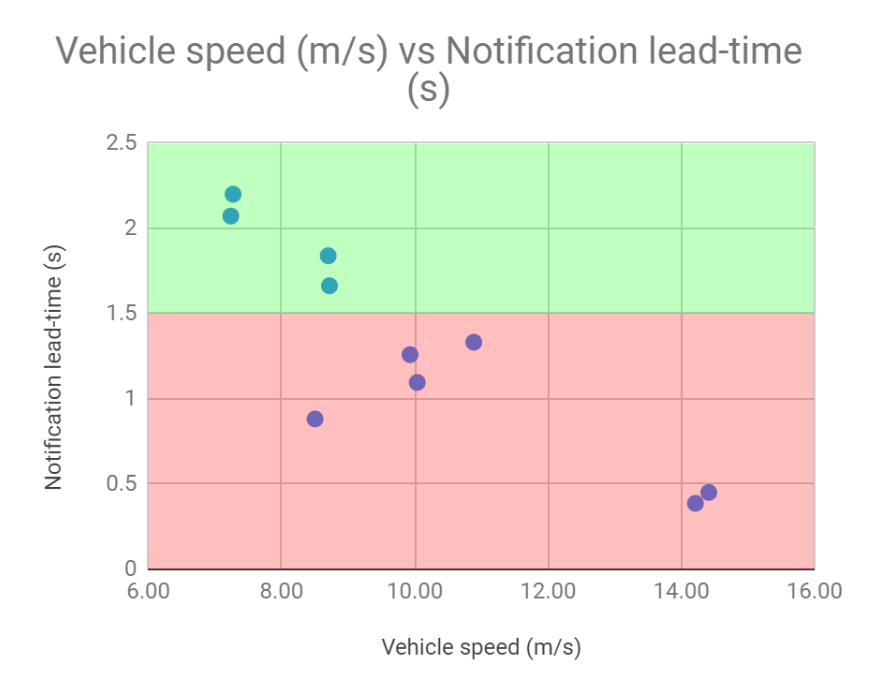
\includegraphics[width=\columnwidth]{images/BS1_vib.png}
    \caption{Blind spot notification testing data}
    \label{fig:bs1_vib}
\end{figure}

It is worth noting that the two high-speed vehicles came in quick succession, each with another vehicle slightly ahead of them on the next lane. This may have affected the system's response time since the system had seen the other vehicles as well and notified the cyclist. We can conclude that the system works better when vehicles have a lower relative speed to the cyclist and when the road is not too congested such that multiple vehicles are in the cyclists' blind spot at the same time. In the latter situation, it is likely that the blind spot alert would be constantly alerting the cyclist anyway due to the number of vehicles passing by, and the presence of the alert is more important than the lead-time.

As for the blind spot notifications, results do not meet initial specifications but are still reasonable. Approximately 39 tests of cars passing further than \SI{2.5}{\meter} to the left were recorded. 33 of these notified the cyclist of a vehicle in the blind spot. Of these, 22 also alerted the cyclist. The specification was to have no alerts.

Nonetheless, the results are still reasonable because the notification persistence time of vehicles at a larger left offset distance is significantly shorter than for vehicles at a shorter offset distance (Fig.~\ref{fig:bs1_pers}). In fact, the maximum persistence time for offset distance above \SI{2.5}{\meter} in 33 tests was \SI{0.769}{\s} with an average of \SI{0.42}{\s}, while for offset distance below \SI{2.5}{\meter}, the persistence time ranges from \SI{0.7}{\s} to \SI{4.45}{\s} with an average of \SI{2.25}{\s}. Given the large difference in notification persistence, it is likely that the cyclist would be over time learn to tell the difference between a vehicle passing close and a vehicle passing far given the length of the alert, albeit at a reduced reaction time.

\begin{figure}
    \centering
    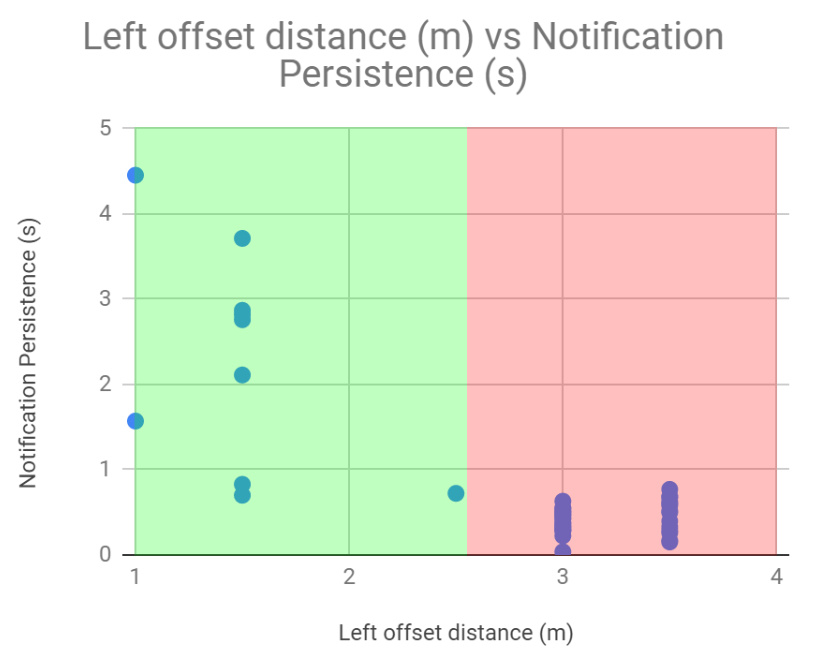
\includegraphics[width=\columnwidth]{images/BS2_persistence.png}
    \caption{Notification persistence testing data}
    \label{fig:bs1_pers}
\end{figure}

\subsection{Proximity Warnings}
The proximity warning tests were very successful. In all 6 tests, when a vehicle passed within \SI{2.5}{\meter} of the left of the bicycle, the proximity lights were activated.

\section{Related Work}
There are not many projects that make a serious attempt to build a full-scale bicycle safety system like CycleSafe. Some related work include a bicycle blind spot detection system \cite{bicycle_blind_spot}, which consisted of an ultrasonic sensor on the back of the helmet and LED notification about nearby cars. Another project called Sixth Sense \cite{bicycle_sixth_sense} is a wireless distance sensor that vibrates a smart device when objects, such as cars, are nearby. These projects only have very limited functionality with car detection, especially when cars are approaching at faster speeds, since the range of their distance sensors is small, and it does not seem like they have acceleration detection.

Most of the safety features of CycleSafe were inspired by current car safety features. For example Honda Sensing \cite{honda_safety}, which is a suite of safety features included on consumer Honda cars, now includes the following safety features
\begin{itemize}
    \item Collision Mitigation Braking System
    \item Road Departure Mitigation
    \item Blind Spot Information System
\end{itemize}
CycleSafe focuses on implementing collision avoidance and blind spot information.

\section{Summary}
CycleSafe provides a comprehensive safety system that makes biking safer than current biking practices, by giving the rider warnings well ahead of collisions with cars and objects that come from behind, to the side, and in front of the rider. In addition, CycleSafe illuminates the rider with LEDs that help make the rider much more visible on the road than current bicycle lights do. By keeping cyclists and drivers more alert of each other on the road, CycleSafe can prevent many of the fatal cyclist accidents that occur every year.

\subsection{Future Work}
The rigid placement of sensors was good for accurate measurements of far-away objects when the road was flat, but whenever we faced non-flat roads, the sensors would point in slightly-off directions that compromised the effectiveness of the system. For example, while going down hills, the front LIDAR would tilt towards the ground, which made CycleSafe believe the rider was about to crash into the ground, when in reality the rider is just facing at an angle below the horizontal. In order to resolve this issue, we have considered solutions that can make the sensors on the bicycle adjustable. For example, by attaching all the sensors to actuators and servos, the LIDAR and ultrasonic sensors can be tuned to the correct position by detecting the difference in the bicycle position to the horizontal plane. An adjustable sensor array would also be useful if the system wanted to collect multiple data points, instead of just single distances from each sensor. Having more data points in a 3D space could help build a more comprehensive picture of the cyclist's surroundings, and improve recognition of dangerous situations.

Another issue we faced was a good deal of false alerts for frontal collision with obstacles that had no threat to the rider. For example, whenever the rider would turn the bicycle suddenly, sweeping the LIDAR across an obstacle quickly, even if the obstacle was not going to be hit would trigger the buzzers (e.g. turning your bicycle around while stationary). The reason is that CycleSafe is unaware that the bicycle is turning, and from the system's perspective an obstacle has suddenly appeared in front of the cyclist. However, since the time facing the obstacle is only momentary, it would be useful if CycleSafe had some way of knowing the obstacle did not pose a hazard. Some solutions that we could implement to improve the collision detection is to add a compass to the system as well as a mechanism to detect turning of the handlebars, and add actuators to the frontal sensor array, allowing the system to look ahead at the cyclist's path during a turn. The design challenges here, however, are out of the scope of this project.

Finally, since we only constructed a prototype for our bicycle, we would like to build CycleSafe with stronger materials and higher quality electronics. For example, all of our circuits could be printed on PCBs, and the casing for our sensors could be in metal instead of acrylic. In addition, since we were not able to waterproof the bicycle sensor array, we would find ways to waterproof that aspect as well, so CycleSafe could be used in rainy weather conditions. 

\subsection{Lessons Learned}
The biggest problem we encountered during this project was that the parts we ordered did not come in on time, even if they are ordered through Amazon Prime. We learned to cope with the additional delivery time by planning other work to do while waiting for parts to come in. In addition, we found that testing was very cumbersome due to the overhead in restarting our system whenever it crashed. Building in more descriptive debugging hooks and software capabilities to recover from crashes are good ways to make the testing process more efficient.

A second problem we encountered was the the problem with outdated Android app development guides and legacy code that required a lot of debugging and tweaking in order to work on modern versions of Android Studio. Backwards compatibility for plugins and Gradle scripts would have made it easier for us to develop the app.

% use section* for acknowledgment
\section*{Acknowledgment}
The CycleSafe team would like to thank the Electrical and Computer Engineering Department of Carnegie Mellon University for their financial support in making this project possible. In addition, we would like to thank Professor Ken Mai for his advising throughout the project
and Zilei Gu for being our TA and her constant support and check-ins with our team.


% trigger a \newpage just before the given reference
% number - used to balance the columns on the last page
% adjust value as needed - may need to be readjusted if
% the document is modified later
%\IEEEtriggeratref{8}
% The "triggered" command can be changed if desired:
%\IEEEtriggercmd{\enlargethispage{-5in}}

%% BIBLIOGRAPHY
\bibliographystyle{IEEEtran}
\bibliography{biblio}

\clearpage
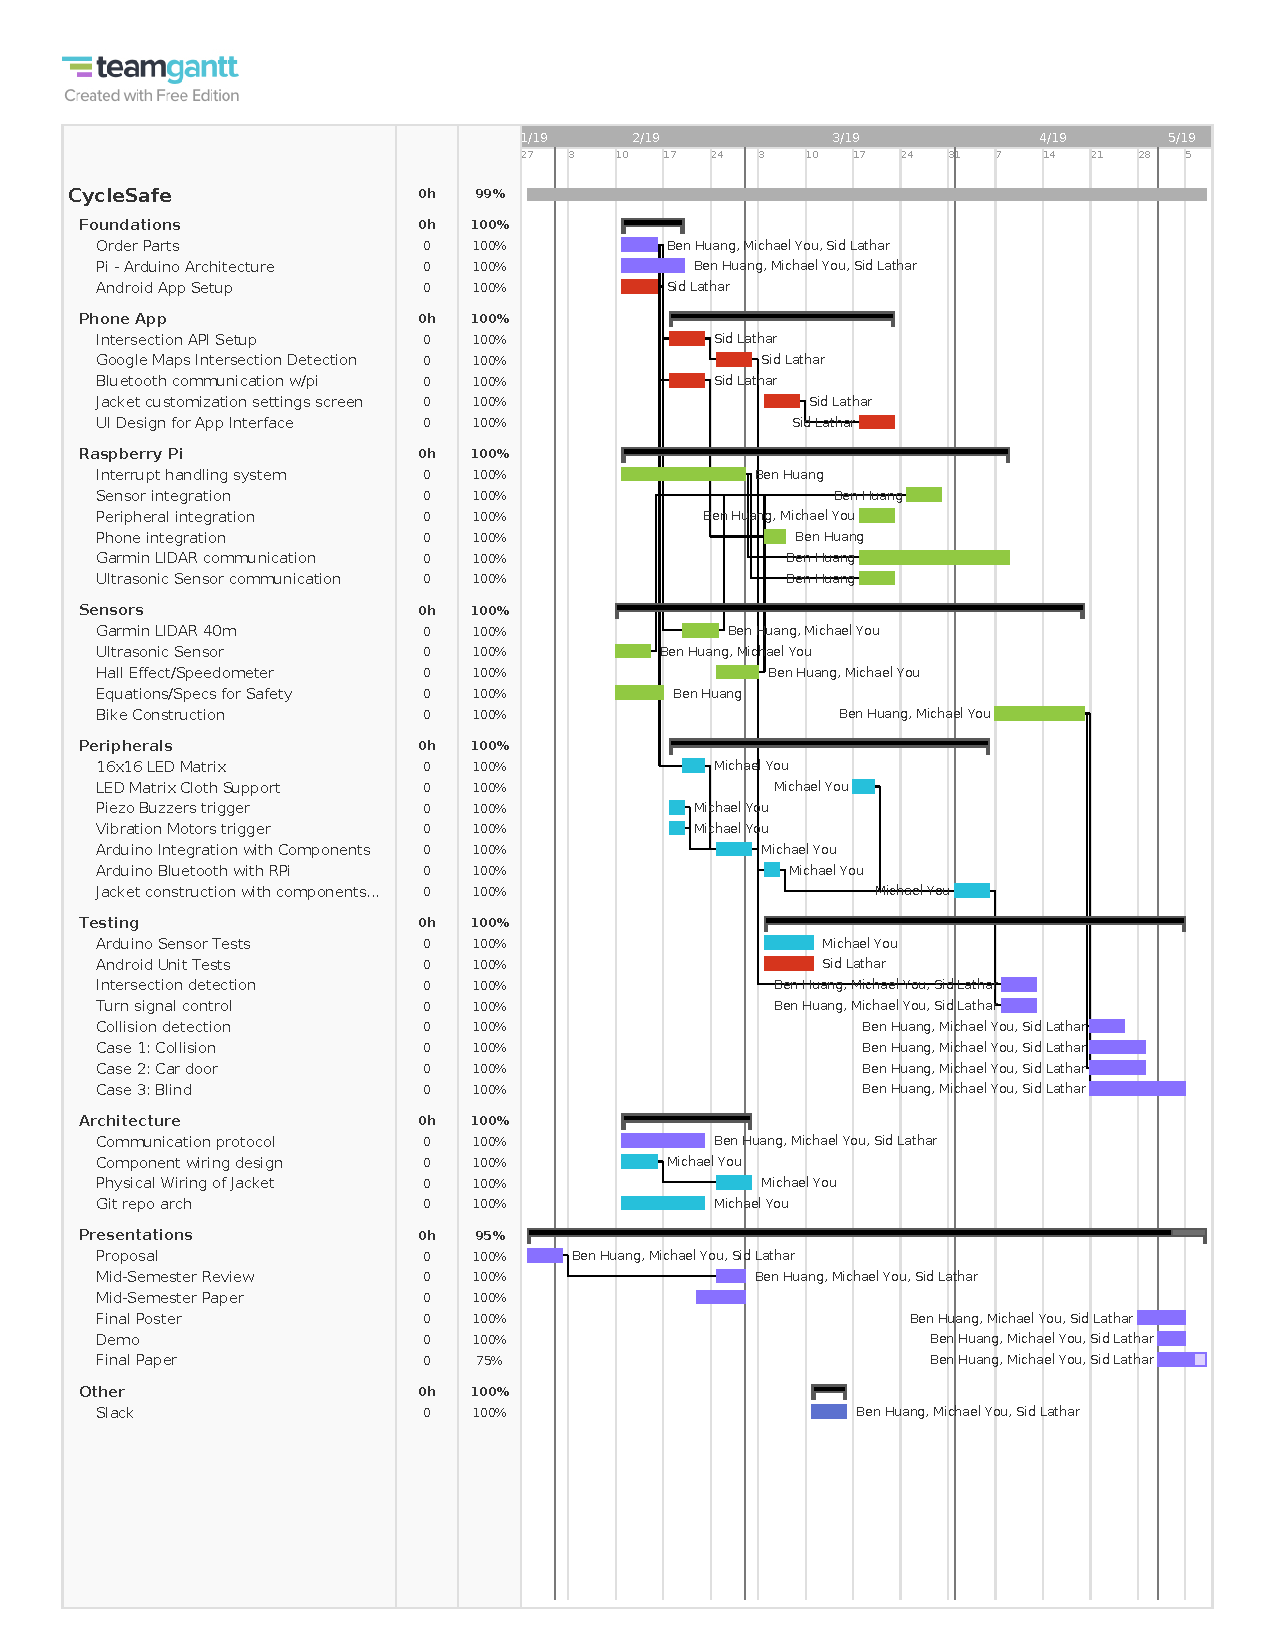
\includepdf[pages=-]{gantt.pdf}

\end{document}


